\section{Marco te\'orico}
\label{sec:marco_teorico}
    %Parrafo 1
    Para avanzar en nuestro proyecto, conforme a los \textbf{Objetivos espec\'ificos} previamente definidos, 
        es esencial comprender los fundamentos de los \textit{aut\'omatas celulares}, incluyendo sus caracter\'isticas 
        y propiedades. Esta comprensi\'on es clave para su implementaci\'on en nuestro proyecto. Por ello, dedicaremos 
        esta secci\'on a detallar estos conceptos b\'asicos, caracter\'isticas y propiedades de los aut\'omatas celulares. 
        Asimismo, proporcionaremos una introducci\'on al mixomiceto \textit{Physarum polycephalum}, destacando su conexi\'on 
        con los aut\'omatas celulares.
    %Parrafo 2
    \vskip 0.5cm
    Adicionalmente, subrayaremos el papel crucial de la \textit{Raspberry Pi 4}, 
        que se encarga de gestionar el robot y de aplicar el aut\'omata celular. Incluir\'a 
        tambi\'en una descripci\'on concisa de la librer\'ia gr\'afica \textit{Biblioteca Multimedia Simple y R\'apida (Simple amd Fast Multimedia Library, SFML)} (o \textit{Vulkan}), 
        seleccionada para la simulaci\'on del aut\'omata celular.

    % Introduccion a los aut\'omatas celulares y su aplicacion en espacios euclidianos
    \subsection{Introducci\'on a los aut\'omatas celulares} 
    \label{sec:AutomatasCelulares}
    % Parrafo 1
    Primero es necesario conocer la teor\'ia de aut\'omatas y como se relaciona con los aut\'omatas celulares,
        por ello daremos un breve repaso de la teor\'ia de aut\'omatas.
    \vskip 0.5cm
    \subsubsection{Teor\'ia de Aut\'omatas}
    \label{sec:TeoriaAutomatas}
    % Parrafo 1
    La teor\'ia de aut\'omatas es el estudio de dispositivos de c\'alculo abtractos, es decir de las m\'aquinas.\cite{Hopcroft1979}
        Estos aut\'omatas son modelos matem\'aticos fundamentales en el \'area de estudio de las ciencias de la computaci\'on, 
        son usados para entender los procesos de c\'alculo y toma de decisiones. En la teor\'ia de aut\'omatas se estudian
        los aut\'omatas finitos, los aut\'omatas con pila, las m\'aquinas de Turing, los aut\'omatas celulares, etc.
        Los aut\'omatas regulares pueden ser jerarquizados en una jerarqu\'ia de Chomsky\cite{Aranda2006}, que es una jerarqu\'ia de lenguajes formales.
        La cual ser\'ia la siguiente:
        \begin{itemize}
            \item \textbf{Tipo 3 - Gram\'aticas regulares:} Estos generan los lenguajes regulares.
                Estas se restrinjen a producciones de la forma $A \rightarrow a\gamma$ y $A \rightarrow aB$. Son 
                asociados a los aut\'omatas finitos.
            \item \textbf{Tipo 2 - Gram\'aticas libres de contexto:} Estos generan los lenguajes independientes del contexto.
                Estas se restrinjen a producciones de la forma $A \rightarrow \gamma$. Son asociados a los aut\'omatas con pila.
            \item \textbf{Tipo 1 - Gram\'aticas sensibles al contexto:} Estos generan los lenguajes sensibles al contexto.
                Estas se restrinjen a producciones de la forma ${\alpha}A{\beta} \rightarrow {\alpha}{\gamma}{\beta}$. 
                Son asociados a las m\'aquinas de Turing linealmente acotadas (significa que la cinta de la m\'aquina de Turing
                tiene un l\'imite derterminada por un cierto n\'umero entero de veces sobre la longitud de entrada).
            \item \textbf{Tipo 0 - Gram\'aticas irrestrictas:} Estos generan los lenguajes recursivamente enumerables.
                Estas se restrinjen a producciones de la forma ${\alpha}A{\beta} \rightarrow {\delta}$. Son asociados a las m\'aquinas de Turing.
        \end{itemize}
    % Parrafo 2
    \vskip 0.5cm
    En cambio los aut\'omatas celulares, aunque diferentes en estructura y aplicaci\'on a las gram\'aticas formales, 
        tambi\'en son modelos matem\'aticos fundamentales en el \'area de estudio de las ciencias de la computaci\'on
        y forman parte de la teor\'ia de aut\'omatas. Mientras que los aut\'omatas convencionales se centran en el procesamiento 
        secuencial de cadenas de s\'imbolos y operan bas\'andose en estados y transiciones claramente definidos, los aut\'omatas 
        celulares utilizan una red de c\'elulas cuyos estados evolucionan en paralelo, siguiendo reglas locales. Esta diferencia 
        fundamental en su enfoque los hace especialmente adecuados para modelar y explorar fen\'omenos que involucran procesos din\'amicos 
        y patrones espaciales. A pesar de estas diferencias, los aut\'omatas celulares se alinean con los principios fundamentales de la 
        teor\'ia de aut\'omatas en cuanto a la representaci\'on y manipulaci\'on de informaci\'on, ofreciendo una perspectiva m\'as amplia y diversa 
        sobre lo que constituye un \textit{`aut\'omata'} en el contexto de la computaci\'on y el procesamiento de informaci\'on. Su inclusi\'on en la teor\'ia 
        de aut\'omatas subraya la amplitud y la profundidad de este campo, demostrando que la teor\'ia de aut\'omatas no solo se limita a las m\'aquinas 
        y lenguajes formales tradicionales, sino que tambi\'en abarca modelos computacionales m\'as generales y vers\'atiles.
    % Parrafo 2
    \vskip 0.5cm
    Una vez que hemos explicado la teor\'ia de automatas podemos pasar a explicar en mas detalle los aut\'omatas celulares.
    \vskip 0.5cm
    \subsubsection{Aut\'omatas celulares de una dimensi\'on}
\label{sec:AutomatasCel1D}
%Parrafo 1
    Los aut\'omatas celulares de una dimensi\'on consisten de una linea de celdas o estados, cada una con 2 estados posibles, 
        0 o 1, vivo o muerto, etc. Estas celdas se actualizan en cada generaci\'on, de acuerdo a una regla de evoluci\'on, 
        la cual determina el estado de una celda en la siguiente generaci\'on, bas\'andose en el estado de la celda y sus 
        vecinos en la generaci\'on actual. La regla de evoluci\'on se aplica a todas las celdas de la misma manera, y en 
        paralelo, es decir, todas las celdas se actualizan al mismo tiempo. Para ejemplificar esto, se puede ver la Figura
        \ref{fig:automataCelular1D}. En donde tenemos la regla de evoluci\'on 30, de las \textit{Reglas de Wolfram}\cite{Wolfram1959}, o
        \textit{Automatas Celulares Elementales} (Elemental Cellular Automata, ECA), en la cual se puede ver que la celda de la generaci\'on $t+1$ depende
        de la celda de la generaci\'on $t$ y sus vecinos.
        \begin{figure}[h!]
            \centering
            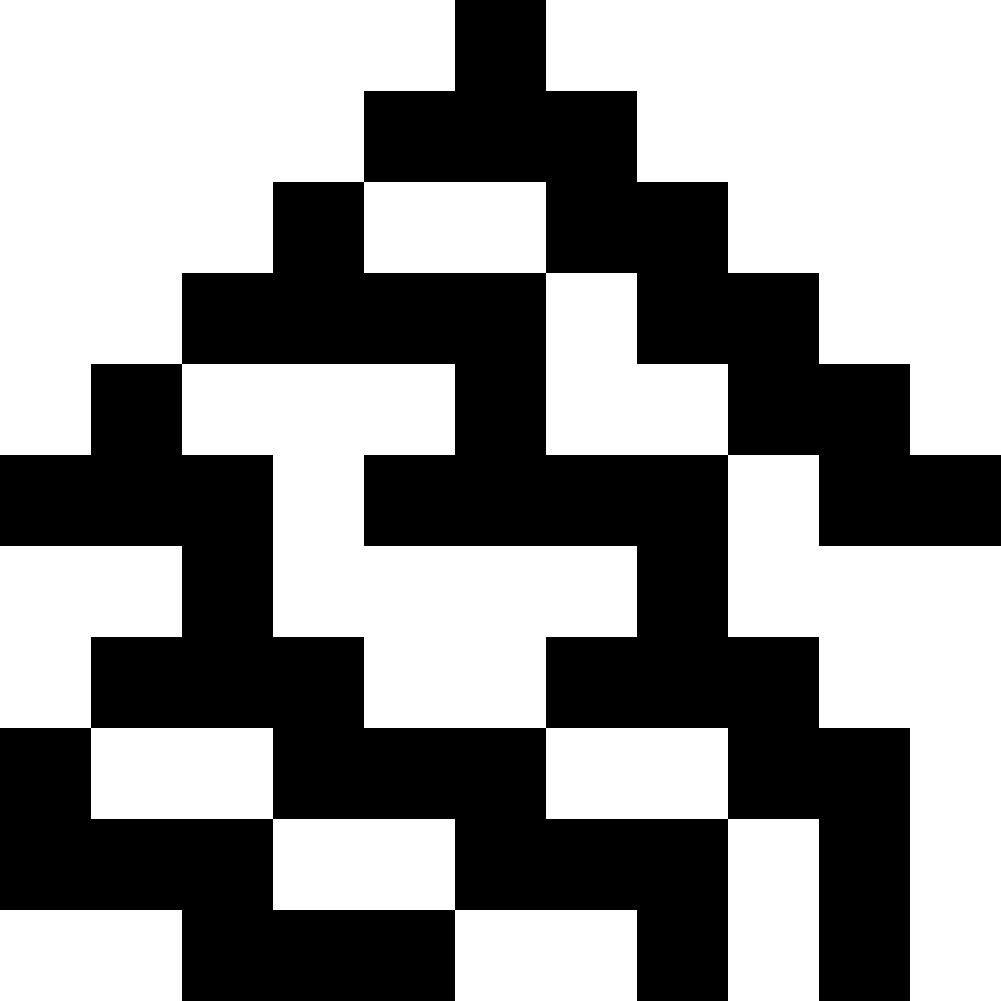
\includegraphics[width=0.5\textwidth]{./images/marco_teorico/automatas_celulares/Regla30.png}
            \caption{Regla de evoluci\'on 30 de las \textit{Reglas de Wolfram} 10 generaciones o (t)}
            \label{fig:automataCelular1D}
        \end{figure}
%Parrafo 2
    \vskip 0.5cm
    Como podemos ver en estos aut\'omatas celulares de una dimensi\'on los que podemos considerar los elementos m\'as importantes son:
        \begin{itemize}
            \item \textbf{Vecindad:} Es el conjunto de celdas que se toman en cuenta para la actualizaci\'on de una celda.
            \item \textbf{Estado:} Es el valor que puede tomar una celda, en este caso solo puede ser 0 o 1.
            \item \textbf{Regla de evoluci\'on:} Es la regla que determina el estado de una celda en la siguiente generaci\'on.
        \end{itemize}
    \vskip 0.5cm
    En este caso la vecindad la forman la celda y sus dos vecinos, pero puede ser de cualquier tama\~no, siempre y cuando
        sea sim\'etrica, es decir, que la celda se encuentre en el centro de la vecindad. El estado de la celda puede ser
        cualquier valor, pero en este caso solo puede ser 0 o 1. La regla de evoluci\'on es la que determina el estado de
        la celda en la siguiente generaci\'on, en este caso la regla de evoluci\'on 30, que se puede ver en la Figura
        \ref{fig:automataCelular1D}, es la siguiente:
        \begin{table}[h!]
            \centering
            \begin{tabular}{|c|c|c|c|c|c|c|c|}
                \hline
                \textbf{111} & \textbf{110} & \textbf{101} & \textbf{100} & \textbf{011} & \textbf{010} & \textbf{001} & \textbf{000} \\
                \hline
                0 & 0 & 0 & 1 & 1 & 1 & 1 & 0 \\
                \hline
            \end{tabular}
            \caption{Regla de evoluci\'on 30}
            \label{tab:reglaEvolucion30}
        \end{table}
    \vskip 0.5cm
    Como podemos ver en el Cuadro \ref{tab:reglaEvolucion30} la regla de evoluci\'on 30 es una regla de evoluci\'on local, 
        es decir, que solo depende de la celda y sus vecinos, y no de toda la l\'inea de celdas. En este caso la regla de evoluci\'on
        30 es una regla de evoluci\'on determinista, es decir, que para una celda y sus vecinos siempre se obtiene el mismo resultado.
        Pero tambi\'en existen las reglas de evoluci\'on no deterministas, en las cuales para una celda y sus vecinos se puede obtener
        m\'as de un resultado. En este caso la regla de evoluci\'on 30 es una regla de evoluci\'on unidimensional, es decir, que la
        celda solo depende de sus vecinos de la izquierda y de la derecha, pero tambi\'en existen las reglas de evoluci\'on
        bidimensionales, n-dimensionales, etc.
    \vskip 0.5cm
    \subsubsection{Condiciones frontera}
        Por definici\'on los aut\'omatas celulares son infinitos, pero en la pr\'actica no se pueden tener aut\'omatas celulares
            infinitos, por lo que se tienen que definir condiciones frontera, las cuales son las condiciones que se tienen en los
            extremos del aut\'omata celular. Existen diferentes tipos de condiciones frontera, las cuales son:
            \vskip 0.5cm
        \begin{wrapfigure}{r}{0.25\textwidth}
            \centering
            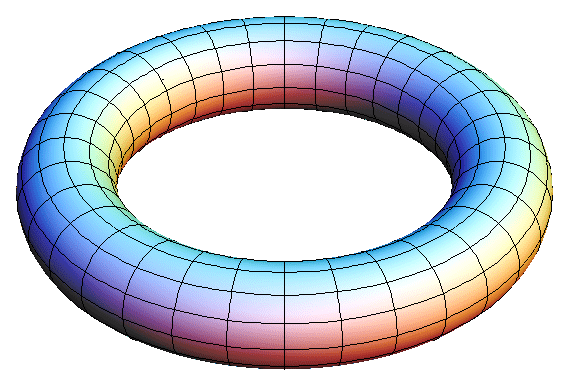
\includegraphics[width=0.25\textwidth]{./images/marco_teorico/automatas_celulares/torus.png}
            \caption{Representaci\'on de un toroide \cite{Sharma2022}}
            \label{fig:toroide}
        \end{wrapfigure}
        \begin{itemize}
            \item \textbf{Abierta} En este caso las celdas de los extremos no tienen vecinos, por lo que no se pueden actualizar.
            \item \textbf{Peri\'odica} En este caso las celdas de los extremos tienen como vecinos a las celdas del otro extremo.
            \item \textbf{Reflejante} En este caso las celdas de los extremos tienen como vecinos a las celdas del otro extremo, pero
                invertidas.
            \item \textbf{Frontera} En este caso las celdas de los extremos tienen como vecinos a celdas con un valor fijo.
        \end{itemize}
    \vskip 0.5cm
    En nuestro caso, utilizaremos la condici\'on frontera peri\'odica; esta tiene forma de un toroide, como se puede ver en la Figura
        \ref{fig:toroide}.
        \vskip 0.5cm
        
        Tambi\'en podemos observar que en la Figura \ref{fig:toroide} se puede ver que las celdas de los extremos tienen como
            vecinos a las celdas del otro extremo, por lo que se puede decir que es una condici\'on frontera peri\'odica.
        \vskip 0.5cm
    \subsubsection{Vecindario}
    \label{sec:Vecindario}
    Un vecindario es un conjunto de celdas que se toman en cuenta para la actualizaci\'on de una celda. Como vimos con anterioridad
        en los aut\'omatas celulares de una dimensi\'on, el vecindario de una celda es la celda y sus dos vecinos, pero en los aut\'omatas
        celulares de dos dimensiones el vecindario de una celda puede ser de cualquier tama\~no, siempre y cuando sea sim\'etrico, es decir,
        que la celda se encuentre en el centro del vecindario. En la Figura \ref{fig:mooreN} se puede ver un ejemplo de un vecindario
        de una celda. E incluso en los aut\'omatas celulares de dos dimensiones se pueden tener vecindarios de diferentes formas, como se
        es com\'un verlos en forma cuadrada y en forma hexagonal, as\'i como se muestra en las Figuras \ref{fig:mooreN} - \ref{fig:hexN}.
    \vskip 0.5cm
    A su vez los vecindarios m\'as usados son los siguientes: 
    \begin{itemize}
        \item 
            \begin{minipage}
                {0.5\textwidth}
                \textbf{Vecindario de Moore} En este caso el vecindario de una celda es la celda y sus ocho vecinos.
            \end{minipage}
            \begin{minipage}{0.5\textwidth}
                \centering
                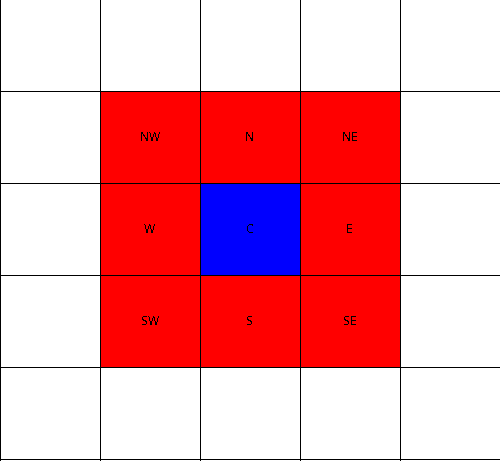
\includegraphics[width=0.5\textwidth]{./images/marco_teorico/automatas_celulares/mooreN.png}
                \captionof{figure}{Vecindario de Moore}
                \label{fig:mooreN}
            \end{minipage}
        \item
            \begin{minipage}
                {0.5\textwidth}
                \textbf{Vecindario de von Neumann} En este caso el vecindario de una celda es la celda y sus cuatro vecinos.
            \end{minipage}
            \begin{minipage}
                {0.5\textwidth}
                \centering
                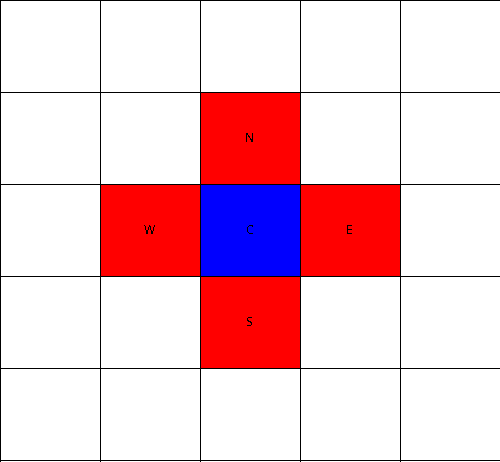
\includegraphics[width=0.5\textwidth]{./images/marco_teorico/automatas_celulares/vonN.png}
                \captionof{figure}{Vecindario de von Neumann}
                \label{fig:vonN}
            \end{minipage}
        \item
            \begin{minipage}
                {0.5\textwidth}
                \textbf{Vecindario de Moore extendido} En este caso el vecindario de una celda es la celda y sus veinticuatro vecinos.
            \end{minipage}
            \begin{minipage}
                {0.5\textwidth}
                \centering
                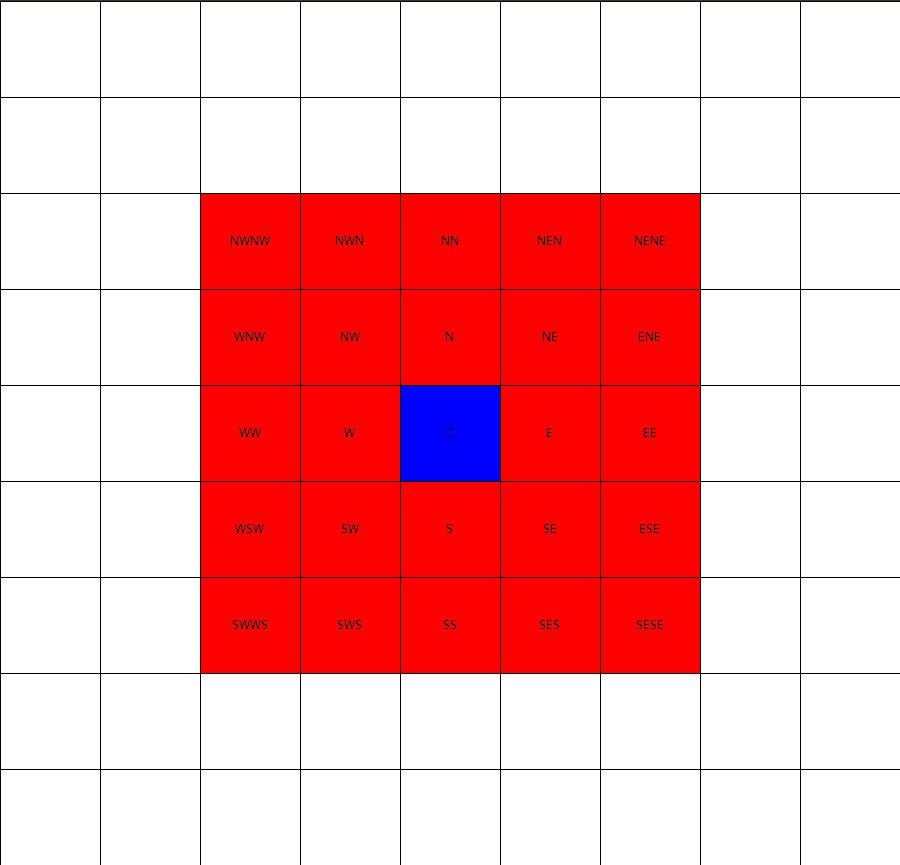
\includegraphics[width=0.5\textwidth]{./images/marco_teorico/automatas_celulares/mooreNeX.jpg}
                \captionof{figure}{Vecindario de Moore extendido}
                \label{fig:mooreNeX}
            \end{minipage}
        \item 
            \begin{minipage}
                {0.5\textwidth}
                \textbf{Vecindario de von Neumann extendido} En este caso el vecindario de una celda es la celda y sus doce vecinos.
            \end{minipage}
            \begin{minipage}
                {0.5\textwidth}
                \centering
                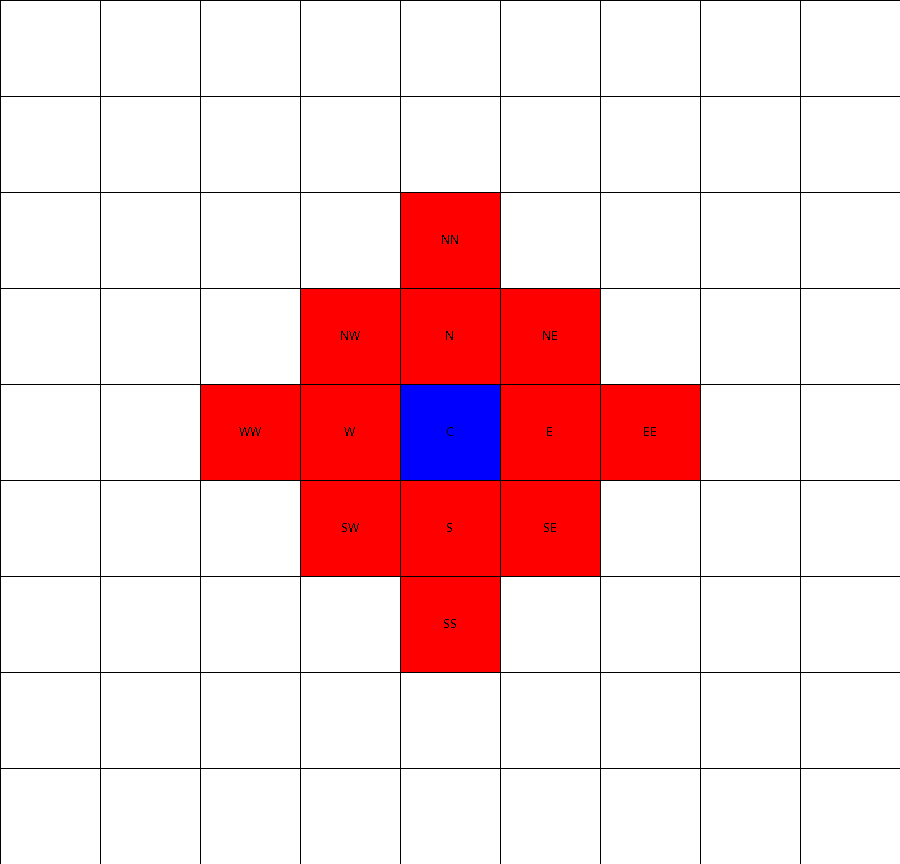
\includegraphics[width=0.5\textwidth]{./images/marco_teorico/automatas_celulares/vonNeX.png}
                \captionof{figure}{Vecindario de von Neumann extendido}
                \label{fig:vonNeX}
            \end{minipage}
        \item
            \begin{minipage}
                {0.5\textwidth}
                \textbf{Vecindario de hexagonal} En este caso el vecindario de una celda es la celda y sus seis vecinos.
            \end{minipage}
            \begin{minipage}
                {0.5\textwidth}
                \centering
                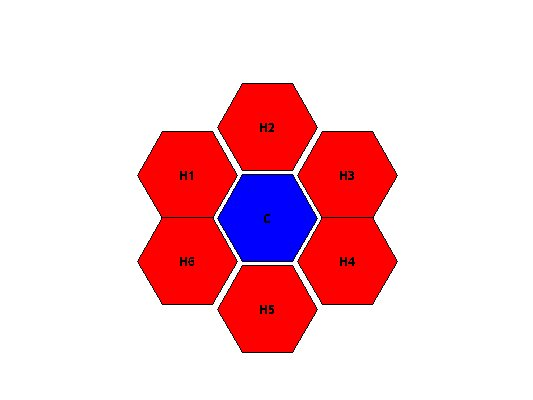
\includegraphics[width=0.5\textwidth]{./images/marco_teorico/automatas_celulares/hexN.jpg}
                \captionof{figure}{Vecindario de hexagonal}
                \label{fig:hexN}
            \end{minipage}
    \end{itemize}
    \vskip 0.5cm
    Una vez que hemos explicado eso podemos pasar a definir formalmente los aut\'omatas celulares.
    \vskip 0.5cm
    \subsubsection{Definici\'on formal}
    \label{sec:AutomatasCelDefFormal}
    Primero denotemos $\mathbb{Z}$ como el conjunto de los n\'umeros enteros, es decir, $\mathbb{Z} = (-\infty,-1 ,0,1, \infty)$.
        y la longitud de cualquier tupla $x$ como $|x|$. Para todas las tuplas $x$ y $y$ de la misma longitud, denotemos $x \oplus y$
        como la tupla que resulta de la suma componente a componente de $x$ y $y$, es decir, $(x \oplus y)_i = x_i + y_i$ para todo 
        $i \in \mathbb{Z}$.
    \vskip 0.5cm
    Entonces tenemos que un aut\'omata celular es una tupla $({\mathbb{Z}^{n}},S,N,f)$ tal que la $n$ dimensi\'on es al menos $1$ donde 
        $n \in \mathbb{Z}^{+}$, $S$ es un conjunto finito no vac\'io de estados, $N$ es un conjunto finito no vac\'io de vecindades 
        perteneciente a ${\mathbb{Z}^{n}}$ y $f$ es una funci\'on de transici\'on local, es decir, $f: S^N \rightarrow S$ donde
        $S^N$ representa al conjunto de todas las posibles configuraciones de vecindad en $N$.
    \vskip 0.5cm
    La configuraci\'on inicial de un aut\'omata celular es una funci\'on $c: {\mathbb{Z}^{n}} \rightarrow S$ que asigna un estado a cada celda.
        La evoluci\'on de un aut\'omata celular es una funci\'on $F: S^{{\mathbb{Z}^{n}}} \rightarrow S^{{\mathbb{Z}^{n}}}$ que asigna una configuraci\'on a la siguiente
        configuraci\'on, es decir, $F(c) = c'$, donde $c'$ es la configuraci\'on resultante de aplicar la funci\'on de transici\'on local a cada
        celda de la configuraci\'on $c$, es decir, $c'(x) = f(c|_{x+N})$ para todo $x \in {\mathbb{Z}^{n}}$, donde $c|_{x+N}$ es la restricci\'on de $c$ a la vecindad $x+N$.
        Esto tambi\'en aplica $n$ dimensionalmente, es decir, que se podr\'ia decir que $c'(x,y) = f(c|_{(x,y)+N})$ para todo $(x,y) \in {\mathbb{Z}^{2}}$.
        Otra notaci\'on que podemos usar, y de hecho es la que utilizaremos es $C(x,y:t)$ donde $C$ es el centro de la vecindad, $x$,$y$ son las coordenadas de la celda y $t$ es el tiempo,
        o generaciones.
    \vskip 0.5cm
    Cabe a\~nadir que puede haber reestricciones adicionales en el conjunto de vecindades $N$ y en la funci\'on de transici\'on local $f$.
        Por ejemplo, en el caso de los aut\'omatas celulares de una dimensi\'on, el conjunto de vecindades $N$ es un conjunto de tuplas de longitud 3,
        donde la primera componente es la celda, la segunda componente es la celda de la izquierda y la tercera componente es la celda de la derecha.
        Y la funci\'on de transici\'on local $f$ es una funci\'on de 8 variables booleanas, es decir, $f: \{0,1\}^3 \rightarrow \{0,1\}$.
    \vskip 0.5cm    
    Y en el caso de los aut\'omatas celulares de dos dimensiones, el conjunto de vecindades $N$ es un conjunto de tuplas de longitud variable, 
        dependiendo del tipo de vecindad, donde la primera componente es la celda y las dem\'as componentes son las celdas vecinas. Por ejemplo, 
        en el caso de la vecindad de Moore, el conjunto de vecindades $N$ es un conjunto de tuplas de longitud 9, donde la primera componente es la celda
        $(x,y)$ el cual ser\'ia el centro de la vecindad, la segunda componente es la celda $(x-1,y-1)$, la tercera componente es la celda $(x-1,y)$,
        la cuarta componente es la celda $(x-1,y+1)$, la quinta componente es la celda $(x,y-1)$, la sexta componente es la celda $(x,y+1)$, la s\'eptima
        componente es la celda $(x+1,y-1)$, la octava componente es la celda $(x+1,y)$ y la novena componente es la celda $(x+1,y+1)$. Aqu\'i 
        $(x,y)$ es la celda central de la vecindad. Y la funci\'on de transici\'on local $f$ es una funci\'on de 512 variables booleanas, es decir,
        $f: \{0,1\}^{9} \rightarrow \{0,1\}$.
    \vskip 0.5cm
    Esta definici\'on formal de aut\'omata celular fue tomada de \cite{Codd1968}. Una vez explicada la definici\'on formal de aut\'omata celular,
        podemos pasar a explicar a m\'as detalle los aut\'omatas celulares de 2 dimensiones, los cuales son los que se usan en este trabajo terminal.
    \vskip 0.5cm
    \subsubsection{Aut\'omatas celulares de 2 Dimensiones}
\label{sec:AutomatasCel2D}

    %Parrafo 1
    Los aut\'omatas celulares de 2 dimensiones son los que se usan en este trabajo terminal, por ello es necesario
        explicarlos con m\'as detalle. Primero recordando lo ya explicado en anteriores subsecciones, un aut\'omata
        celular de 2 dimensiones es una tupla $({\mathbb{Z}^{2}},S,N,f)$\ref{sec:AutomatasCelDefFormal} y este 
        necesita de 8 elementos para poder ser definido, los cuales son los siguientes:         
    \begin{enumerate}
        \item \textbf{Celdas}: Es la unidad b\'asica del aut\'omata celular. Cada celda ocupa una posici\'on en el espacio, 
            para ser representados suelen usarse cuadr\'iculas o redes, esta tiene un estado y una vecindad.
        \item \textbf{Estados}: Cada celda puede estar en uno de varios estados posibles. En los aut\'omatas celulares
            m\'as simples, cada celda puede estar en uno de dos estados posibles (0 o 1, vivo o muerto, etc), pero en los 
            aut\'omatas celulares m\'as complejos, cada celda puede estar en uno de varios estados posibles. En el caso 
            en particular del Physarum polycephalum, cada celda puede estar en uno de nueve estados posibles 
            $\mathbb{P} = \{x \in \mathbb{Z}| 0 \leq x \leq 8\}$ entonces es $S = \mathbb{P}$.
        \item \textbf{Cuadr\'icula o Red}: Las celdas estan dispuestas a lo largo del espacio euclidiano, en 
            suelen ser dispuestas en una cuadr\'icula o red, en donde cada celda ocupa una posici\'on en el espacio. Es
            n-dimensional, pero en este caso es 2-dimensional, es decir, $n = 2$.
        \item \textbf{Vecindad}: Es el conjunto de celdas que se toman en cuenta para la actualizaci\'on de una celda. En el caso de
            la vecindad de Moore que se puede ver en la secci\'on \ref{sec:Vecindario} $N = 8$
        \item \textbf{Reglas de Transici\'on}: Son un conjunto de reglas que determinan como cambia el estado de la celula en 
            funci\'on del estado actual de ella y de sus vecinos. Estas reglas se aplinan repetidamente a lo largo del tiempo,
            generalmente de manera sincr\'ona, es decir, todas las celdas se actualizan al mismo tiempo. Estas estan definidas 
            por la funci\'on de transici\'on local $f$. Ejemplificando lo anterior tenemos que en el juego de la vida de Conway
            \cite{Conway1970} donde tenemos que $C(x,y:t)$ que es la celda central y $N(x,y:t)$ que es la vecindad de Moore de la
            celda central, adem\'as tenemos que tiene $f: \{0,1\}^9 \rightarrow \{0,1\}$, entonces podemos deducir que la funci\'on de transici\'on 
            se define como:
            \begin{equation*}
                f(C(x,y:t),N(x,y:t)) = \begin{cases}
                    1 & \text{si } C(x,y:t) = 0 \text{ y } N(x,y:t) = 3 \\
                    1 & \text{si } C(x,y:t) = 1 \text{ y } N(x,y:t) = 2 \text{ o } N(x,y:t) = 3 \\
                    0 & \text{en otro caso}
                \end{cases}
            \end{equation*}
        \item \textbf{Tiempo o Generaciones}: Es el n\'umero de veces que se aplica la funci\'on de transici\'on local $f$. En este caso
            es $t \in \mathbb{Z}^{+}$. 
        \item \textbf{Condiciones Iniciales}: Antes de que el aut\'omata celular comience a evolucionar, se debe especificar el estado de
            cada celda. En este caso es $c: {\mathbb{Z}^{2}} \rightarrow S$. Estas condiciones iniciales pueden ser aleatorias o no.
        \item \textbf{Condiciones Frontera}: Son las condiciones frontera previamente mencionadas en la secci\'on \ref{sec:AutomatasCel1D}.
    \end{enumerate}
    \vskip 0.5cm
    
    \subsubsection{Ejemplo}
    Una vez que hemos explicado los aut\'omatas celulares de 2 dimensiones podemos pasar a explicar un ejemplo de un aut\'omata celular de 2 dimensiones.
    \vskip 0.5cm
    En este caso mostraremos un aut\'omata celular de 2 dimensiones(binario) con vecindad de Moore y con una configuraci\'on totalistica 
        B4678/S35678, es decir, una celda nacer\'a si tiene 4, 6, 7 u 8 vecinos vivos y sobrevivir\'a si tiene 3, 5, 6, 7 u 8 vecinos vivos.
        Este aut\'omata celular tambi\'en es conocido con el nombre de \textit{Anneal} y es mencionado en \cite{Bastien2010}.
    \vskip 0.5cm
    Para formalizar tenemos que este aut\'omata $\mathbb{A} = (\mathbb{Z}^2, S, N, f)$ donde: 
        $S = \{0,1\}$, $N = \{0,1\}^9$ y $f: \{0,1\}^9 \rightarrow \{0,1\}$ y $C$ es la celda central, 
        entonces podemos deducir que la funci\'on de transici\'on se define como:
        \begin{equation*}
            f(C(x,y,t),N(x,y,t)) = \begin{cases}
                1 & \text{si } C(x,y,t) = 0 \text{ y } N(x,y,t) \in \{4,6,7,8\} \\
                1 & \text{si } C(x,y,t) = 1 \text{ y } N(x,y,t) \in \{3,5,6,7,8\} \\
                0 & \text{en otro caso}
            \end{cases}
        \end{equation*}
    \vskip 0.5cm
    Dandonos como resultado la siguiente evoluci\'on en 250 generaciones:
    \begin{figure}[h]
        \centering
        
\includegraphics[width=0.5\textwidth]{./images/marco_teorico/automatas_celulares/Anneal.png}
        \caption{Evoluci\'on del aut\'omata celular \textit{Anneal}}
        \label{fig:anneal}
    \end{figure}
    \clearpage
    \subsubsection{Entrop\'ia de Shannon}
\label{sec:Entriopia}
    La entrop\'ia de Shannon es un concepto fundamental en la teor\'ia de la informaci\'on, 
        que se utiliza para medir la incertidumbre en una variable aleatoria. La entrop\'ia en si 
        es el grado de informaci\'n/desinformaci\'on que tenemos en un sistema. Es decir que cuanta m\'as
        informaci\'on tengamos de un sistema, menor ser\'a la entrop\'ia y viceversa. La entrop\'ia de Shannon, 
        nombrada as\'i por Claude Shannon\cite{Shannon1948}, se define mate la suma negativa de las probabilidades de cada
        posible valor de la variable aleatoria multiplicada por el logaritmo de la probabilidad de ese valor. Esta
        definici\'on es la siguiente:
        \begin{equation}
            H(X) = -\sum_{i=1}^{n} p(x_i) \log_b p(x_i)
        \end{equation}
    \vskip 0.5cm
    Donde $X$ es una variable aleatoria discreta, $p(x_i)$ es la probabilidad de que la variable aleatoria 
        $X$ tome el valor $x_i$ y $b$ es la base del logaritmo. En el caso de que la base del logaritmo sea 2, 
        la unidad de medida de la entrop\'ia ser\'an los bits. En el caso de que la base del logaritmo sea $e$,
        la unidad de medida de la entrop\'ia ser\'an los nat. Y en el caso de que la base del logaritmo sea 10, 
        la unidad de medida de la entrop\'ia ser\'an los dits.
    \vskip 0.5cm
    En nuestro caso en particular usamos bits como unidad de medida de la entrop\'ia, ya que lo usamos para saber que tipo de comportamiento
        tiene el aut\'omata celular. Es decir, si la entrop\'ia es alta, entonces el aut\'omata celular tiene un comportamiento ca\'otico, y si 
        la entrop\'ia es baja, entonces el aut\'omata celular tiene un comportamiento ordenado.
    \vskip 0.5cm
    Como vimos en ejemplo anterior, el aut\'omata celular \textit{Anneal} podemos observar r\'apidamente su entrop\'ia
        en la figura \ref{fig:annealEntropia}: 
        \begin{figure}[h]
            \centering
            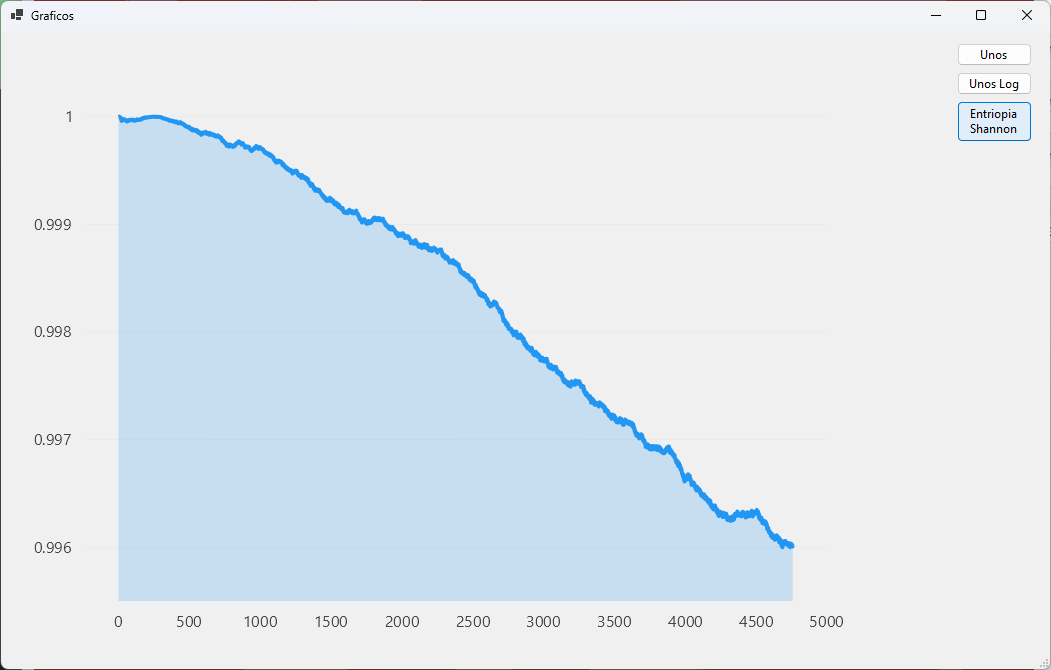
\includegraphics[width=0.5\textwidth]{./images/marco_teorico/automatas_celulares/Anneal5kShann.png}
            \caption{Entrop\'ia del aut\'omata celular \textit{Anneal} en 5000 generaciones}
            \label{fig:annealEntropia}  
        \end{figure}
    \subsubsection{Sistemas Din\'amicos}
\label{sec:SistemasDinamicos}
    La teor\'ia de Sistemas Din\'amicos puede considerarse una forma de describir c\'omo un determinado estado
        se transforma o evoluciona en otro a lo largo del tiempo, es decir, c\'omo evoluciona un sistema en el tiempo.
        La teor\'ia de Sistemas Din\'amicos se puede aplicar a cualquier \'area de la ciencia, como por ejemplo,
        la biolog\'ia, la econom\'ia, la f\'isica, la qu\'imica, etc. En nuestro caso en particular, la teor\'ia de
        Sistemas Din\'amicos se aplica a los aut\'omatas celulares, ya que los aut\'omatas celulares son sistemas
        din\'amicos discretos.
    \vskip 0.5cm
    Nos referimos a sistemas din\'amicos discretos cuando el tiempo es discreto. Con los aut\'omatas celulares
        podemos ver que el tiempo es discreto, ya que el tiempo se mide en generaciones. Es decir, en cada generaci\'on
        el aut\'omata celular evoluciona de un estado a otro. En la Figura \ref{fig:automataCelularEvolucion} podemos
        ver un ejemplo de la evoluci\'on de un aut\'omata celular en el tiempo:
        \begin{figure}[h]
            \centering
            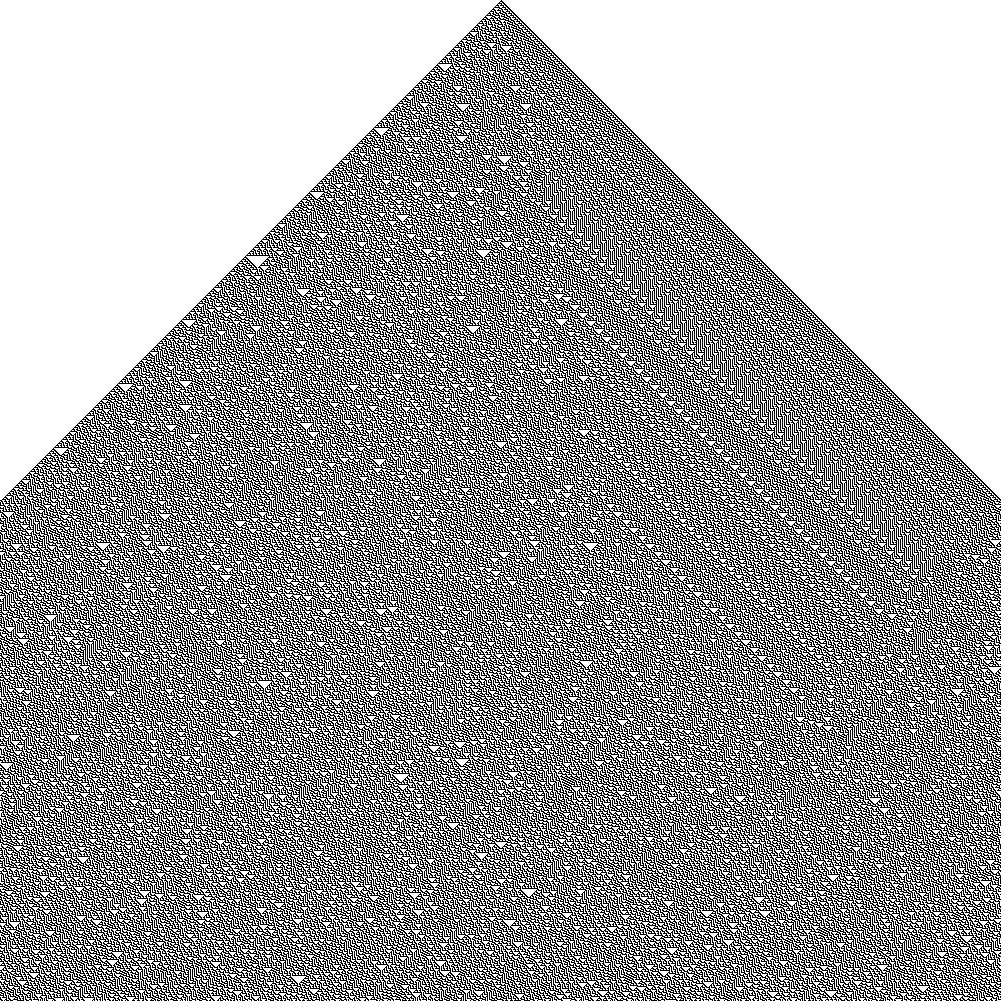
\includegraphics[width=0.5\textwidth]{./images/marco_teorico/automatas_celulares/Regla30-1000Gen.png}
            \caption{Evoluci\'on de la regla 30 en 1000 generaciones o pasos de tiempo}
            \label{fig:automataCelularEvolucion}
        \end{figure}
    \vskip 0.5cm
    No daremos una explicaci\'on m\'as en profundidad de los sistemas din\'amicos, ya que no es el objetivo de este
        trabajo. Para m\'as informaci\'on sobre sistemas din\'amicos y caos, se recomienda leer \cite{Ott1993} y tambi\'en \cite{Luenberger1979}.
        Sin embargo, lo que s\'i es importante mencionar es que los sistemas din\'amicos pueden ser clasificados,
        en este caso nos enfocaremos en los sistemas triviales, los sistemas complejos y los sistemas ca\'oticos.
    \vskip 0.5cm
    Esto lo hacemos con el prop\'osito de poder clasificar el comportamiento de nuestro aut\'omata celular (Physarum Polycephalum)
        en base a su comportamiento. Es decir, si el aut\'omata celular se comporta de manera trivial, compleja o ca\'otica.
        Para esto, primero daremos una breve explicaci\'on de cada uno de estos tipos de sistemas din\'amicos. A su vez, 
        quisi\'eramos destacar que para hacer nuestra clasificaci\'on o determinar el tipo de comportamiento tiene nuestro aut\'omata
        celular usaremos una gr\'afica en la cual podamos observar la Entrop\'ia de Shannon en funci\'on del tiempo. Ya que para
        poder usar como m\'etodo de clasificaci\'on los atractores, requerimos que la cantidad de estados en el Physarum Polycephalum
        es: $\mathbb{P} = \{x \in \mathbb{Z}| 0 \leq x \leq 8\}$ entonces es $S = \mathbb{P}$ y por lo tanto su funci\'on de transici\'on es: 
        $f: \mathbb{P} \rightarrow \mathbb{P}$ o sea $f: \mathbb{P}^{N} \rightarrow \mathbb{P}$ donde $N$ es la vecindad del aut\'omata celular.
        Por lo tanto, la funci\'on de transici\'on es una funci\'on de $\mathbb{P}^{9}$, 
        dandonos como resultado un total de $9^{9}$ o sea 387,420,489 estados posibles. Por lo tanto, no es posible graficar todos los
        estados posibles del aut\'omata celular.
    \vskip 0.5cm
    Ahora si, daremos una breve explicaci\'on de los sistemas mencionados anteriormente:
    \begin{itemize}
        \item \textbf{Sistemas Triviales:} Son sistemas que no tienen comportamiento complejo, es decir, son sistemas que
            tienen un comportamiento predecible. Por ejemplo, un p\'endulo simple, ya que su movimiento es peri\'odico y predecible.
        \item \textbf{Sistemas Complejos:} Son sistemas que tienen un comportamiento complejo, es decir, son sistemas que
            tienen un comportamiento impredecible debido a su sensibilidad a las condiciones iniciales y a la presencia de interacciones no 
            lineales.  Por ejemplo, el clima, ya que es imposible predecir el clima con exactitud.
        \item \textbf{Sistemas Ca\'oticos:} Los sistemas ca\'oticos son un subconjunto de sistemas complejos que son extremadamente sensibles 
            a las condiciones iniciales. Peque\~nas variaciones en las condiciones iniciales pueden llevar a resultados completamente diferentes en el
            tiempo. Los sistemas ca\'oticos pueden parecer aleatorios y desordenados, pero en realidad est\'an gobernados por ecuaciones matem\'aticas 
            deterministas. Un ejemplo cl\'asico de sistema ca\'otico es el sistema de doble p\'endulo, donde el movimiento se vuelve impredecible y 
            altamente sensible a las condiciones iniciales despu\'es de un corto per\'iodo de tiempo.
    \end{itemize}

    % Introduccion al Physarum Polycephalum
    \subsection{Physarum Polycephalum}
    \label{sec:PhysarumPolycephalum}
    % Parrafo 1
    Para poder desarrollar este Trabajo Terminal es necesario conocer el organismo que se va a modelar, 
        en este caso el Physarum Polycephalum. Por lo tanto, en esta secci\'on daremos una breve introducci\'on
        al Physarum Polycephalum, as\'i como sus caracter\'isticas y propiedades.
    \vskip 0.5cm
    % Parrafo 2
    \subsubsection{Mixomiceto}
    Los mixomicetos, tambi\'en conociods como myxo-mycetes o mohos mucilaginosos, son 
        un grupo de organismos unicelulares que se encuentran en el reino Protista.
        A pesar de su apariencia poco llamativa y su tama\~no microsc\'opico,
        los mixomicetos son organismos muy interesantes, por su ciclo de vida y su comportamiento
        biol\'ogico inusual.
    \vskip 0.5cm
    A diferencia de las setas y otros hongos tradicionales, los mixomicetos no forman estructuras 
        multicelulares visibles durante la mayor parte de su ciclo de vida. En su lugar, 
        existen como c\'elulas individuales, generalmente microsc\'opicas, que se desplazan 
        a trav\'es de ambientes h\'umedos y ricos en materia org\'anica y condiciones 
        favorables para su crecimiento.
    \vskip 0.5cm
    % Parrafo 3
    Los mixomicetos toman 3 formas distintas durante el transcurso de su vida: 
    \begin{itemize}
        \item \textbf{Amoeboides}: Son c\'elulas individuales que se mueven por medio de 
            seud\'opodos o flagelos dependiendo principalmente de la cantidad de agua en el medio.
            Estas amebas se denominan \textit{myxamoebas} y son las que se encuentran en el suelo.
        \item \textbf{Plasmodio}: Es una masa de citoplasma multinucleado sin separaci\'on de 
            membranas celulares, que se mueve por medio de la contracci\'on de sus fibras de actina.
            Este plasmodio es el que se encuentra en el interior de los troncos de los \'arboles.
        \item \textbf{Cuerpo fruct\'ifero}: Es la estructura que se forma cuando el plasmodio 
            se transforma en esporas. Estas esporas son las que se encuentran en la parte superior 
            de los troncos de los \'arboles.
    \end{itemize}
    \vskip 0.5cm
    % Parrafo 4
    \subsubsection{Ciclo de vida}
    El ciclo de vida de los mixomicetos es muy complejo, y se divide en dos fases: 
        la fase vegetativa y la fase reproductiva.
    \vskip 0.5cm
    % Parrafo 5
    La fase vegetativa se divide en 3 etapas:
    \begin{itemize}
        \item \textbf{Etapa de alimentaci\'on}: En esta etapa, las c\'elulas individuales 
            se mueven por medio de seud\'opodos o flagelos, y se alimentan de bacterias, 
            levaduras y otros microorganismos que se encuentran en el suelo.
        \item \textbf{Etapa de crecimiento}: En esta etapa, las c\'elulas individuales 
            se fusionan para formar un plasmodio, que es una masa de citoplasma multinucleado 
            sin separaci\'on de membranas celulares, que se mueve por medio de la contracci\'on 
            de sus fibras de actina.
        \item \textbf{Etapa de maduraci\'on}: En esta etapa, el plasmodio se transforma en 
            esporas, que son las que se encuentran en la parte superior de los troncos de los \'arboles.
    \end{itemize}
    \vskip 0.5cm
    % Parrafo 6
    La fase reproductiva se divide en 2 etapas:
    \begin{itemize}
        \item \textbf{Etapa de dispersi\'on}: En esta etapa, las esporas se dispersan por 
            medio del viento, y se posan en el suelo.
        \item \textbf{Etapa de germinaci\'on}: En esta etapa, las esporas germinan y se 
            convierten en c\'elulas individuales, que se mueven por medio de seud\'opodos 
            o flagelos, y se alimentan de bacterias, levaduras y otros microorganismos 
            que se encuentran en el suelo.
    \end{itemize}
    \vskip 0.5cm
    % Parrafo 7
    El ciclo de vida de los mixomicetos se puede observar en la figura \ref{fig:MixomicetoCicloVida}.
    \begin{figure}[h]
        \centering
        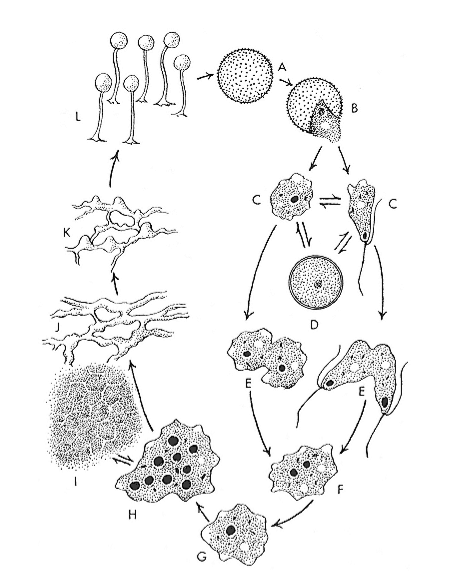
\includegraphics[width=0.5\textwidth]{./images/marco_teorico/Physarum/mixomiceto_ciclo_vida.png}
        \caption{Ciclo de vida de los mixomicetos.}
        \label{fig:MixomicetoCicloVida}
    \end{figure}
    \vskip 0.5cm
    % Parrafo 8
    Si desea profundizar en el tema, puede consultar el libro "Myxomycetes: Biology, Systematics, Biogeography, and Ecology" de Rojas \cite{Rojas2017}.
    \vskip 0.5cm
    \subsubsection{Physarum Polycephalum}
\label{ssub:PhysarumPolycephalum01}
    %Parrafo 1
    El Physarum Polycephalum, tambi\'en conocido como "The Blob", 
        o "La Mancha", es un protista con formas celulares diversas. El Physarum Polycephalum
        es un mixomiceto acelular, esto proviene de la etapa plasmoidal de su ciclo de vida,
        en la cual el plasmodio es un coenocito multinucleado macroscopico de color amarillo 
        brillante, formado en una red de tubos entrelazados. Esta etapa del ciclo de vida es 
        la que se utiliza para el estudio de este organismo.\cite{Dee1960} Podemos ver un ejemplo
        en la siguiente Figura \ref{fig:PhysarumPolycephalum01}.
    \begin{figure}[h]  
        \centering
        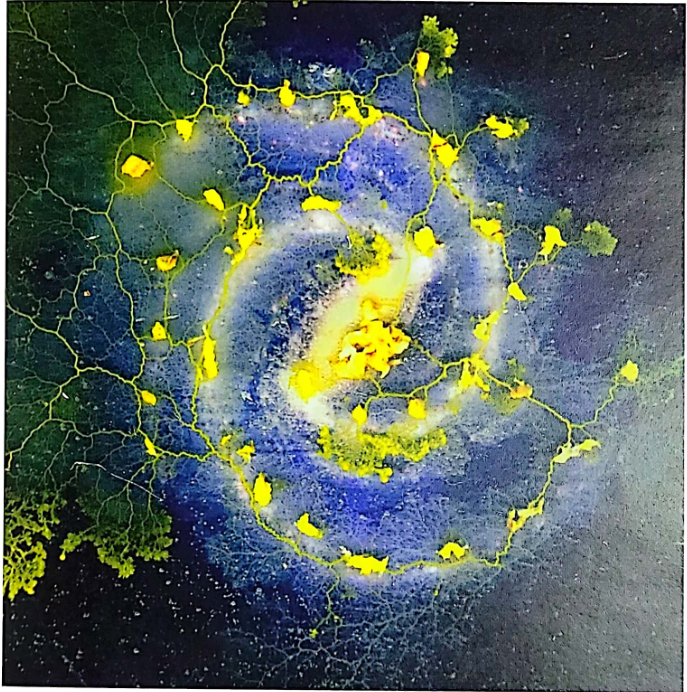
\includegraphics[width=0.5\textwidth]{./images/marco_teorico/Physarum/PhyrasumPolycephalum01.png}
        \caption{Physarum propag\'andose en una impresi\'on art\'istica de una galaxia. Imagen extra\'ida de 'Atlas of Physarum Computing' de A. Adamatzky \cite{Adamatzky2014}.}
        \label{fig:PhysarumPolycephalum01}
    \end{figure} 
    \vskip 0.5cm
    %Parrafo 2
    Como vimos con anterioridad, los mixomicetos se dividen en dos etapas, el plasmodio y los cuerpos fruct\'iferos.
        El Physarum Polycephalum es un mixomiceto que se encuentra en la etapa plasmodial de su ciclo de vida, 
        en la cual el plasmodio es un coenocito multinucleado macroscopico de color amarillo brillante, formado en una red de tubos entrelazados.
        Esta etapa del ciclo de vida es la que se utiliza para el estudio de este organismo.\cite{Dee1960}
    \begin{wrapfigure}{r}{0.17\textwidth}
        \centering
        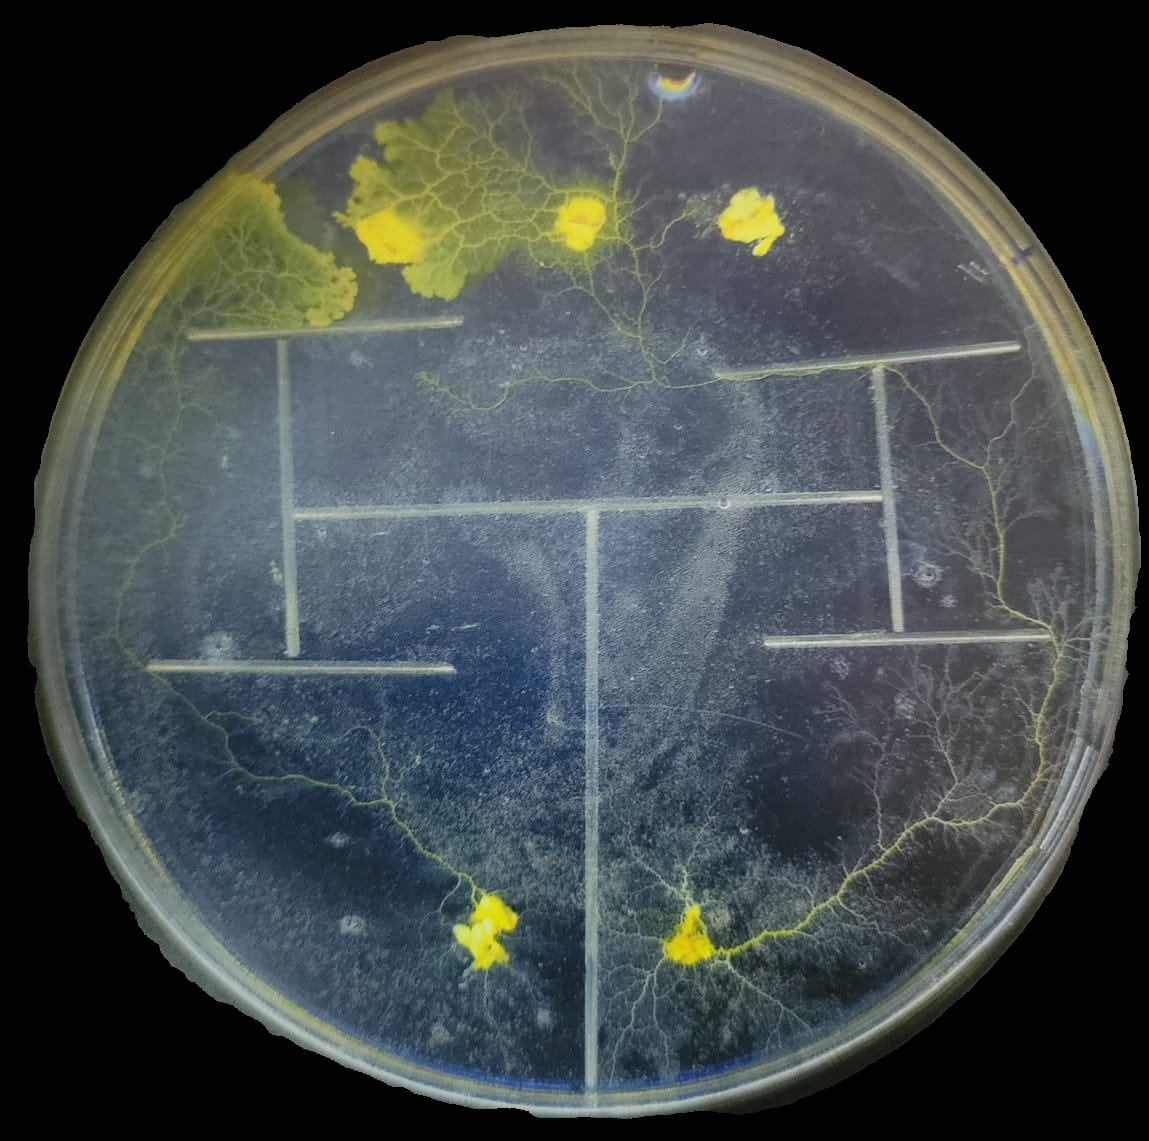
\includegraphics[width=0.17\textwidth]{./images/marco_teorico/Physarum/LaberintoPhysarum.png}
        \caption{Physarum Polycephalum resolviendo un laberinto. \cite{Adamatzky2014}.}
        \label{fig:PhysarumPolycephalum02}
    \end{wrapfigure}
    \vskip 0.5cm
    %Parrafo 3
    El Physarum Polycephalum es un organismo que se encuentra en la naturaleza en lugares h\'umedos y oscuros, 
        como en el interior de los troncos de los \'arboles en descomposici\'on, en hojarasca h\'umeda, en suelos 
        ricos en materia org\'anica y en lugares oscuros y h\'umedos. Este organismo se alimenta de bacterias, 
        hongos y otros microorganismos que se encuentran en su entorno, y se desplaza por medio de la contracci\'on 
        de sus fibras de actina, que le permiten moverse en busca de alimento.\cite{Dee1960}
    \vskip 0.5cm
    %Parrafo 4
    El Physarum Polycephalum es un organismo muy interesante para el estudio de la biolog\'ia y la f\'isica, 
        ya que tiene propiedades \'unicas que lo hacen un organismo muy especial. Por ejemplo, el Physarum Polycephalum 
        es capaz de resolver laberintos como se observa en la Figura \ref{fig:PhysarumPolycephalum02}, encontrar la ruta m\'as corta entre dos puntos, y tomar decisiones complejas 
        basadas en la informaci\'on que recibe de su entorno. Adem\'as, el Physarum Polycephalum es capaz de aprender 
        y recordar informaci\'on, y de adaptarse a su entorno de una manera muy eficiente.
    \vskip 0.5cm
    %Parrafo 5
    Una vez dada una breve introducci\'on al Physarum Polycephalum, podemos pasar a la perspectiva de la computaci\'on, 
        en donde el Physarum Polycephalum ha sido utilizado para resolver problemas de optimizaci\'on, simulaci\'on 
        de redes de transporte, y modelado de sistemas complejos. En la siguiente secci\'on veremos c\'omo el Physarum 
        Polycephalum ha sido utilizado en la computaci\'on y en la modelaci\'on de sistemas complejos.
    
    \subsubsection{El Physarum Polycephalum visto desde la perspectiva computacional}
    % Parrafo 1
    Como se mencion\'o en la secci\'on \ref{ssub:PhysarumPolycephalum01}, el Physarum Polycephalum es un organismo notable 
        que ha despertado un gran inter\'es por parte de bi\'ologos y matem\'aticos debido a su notable capacidad para exhibir comportamientos 
        emergentes y resolver problemas de optimizaci\'on de manera eficiente, demostrando una gran versatilidad. Entre sus comportamientos 
        complejos se encuentran la locomoci\'on, la formaci\'on de redes adaptativas y la toma de decisiones descentralizadas.
    \vskip 0.5cm
    % Parrafo 2
    En la computaci\'on, el Physarum Polycephalum ha sido utilizado para resolver problemas de optimizaci\'on, 
        simulaci\'on de redes de transporte, y modelado de sistemas complejos. En particular, el Physarum Polycephalum
        ha sido utilizado para resolver problemas de optimizaci\'on de rutas, como el problema del camino m\'as corto,
        el problema del flujo m\'aximo, y el problema de la cobertura de sensores. Adem\'as, el Physarum Polycephalum
        ha sido utilizado para modelar sistemas complejos, como la formaci\'on de redes de transporte, la formaci\'on
        de patrones en sistemas biol\'ogicos, y la formaci\'on de estructuras en sistemas f\'isicos.
    \vskip 0.5cm
    % Parrafo 3
    Por mencionar algunos ejemplos de aplicaciones del Physarum Polycephalum en la computaci\'on, tenemos los siguientes:
    \begin{itemize}
        \item \textbf{A physarum-inspired prize-collecting steiner tree approach to identify subnetworks for drug repositioning}:
            En el art\'iculo se detalla c\'omo un algoritmo, inspirado en el moho Physarum polycephalum, se aplica para descubrir medicamentos 
            que podr\'ian ser \'utiles en el tratamiento de enfermedades cardiovasculares. Mediante la construcci\'on de Redes de Similitud de F\'armacos 
            (Drug Similarity Networks, DSNs), donde los nodos representan medicamentos y las conexiones reflejan similitudes entre ellos basadas en caracter\'isticas como la 
            estructura qu\'imica y los efectos terap\'euticos, cada medicamento recibe un 'premio' seg\'un su similitud con otros ya utilizados en afecciones 
            cardiovasculares. El algoritmo busca dentro de estas redes para encontrar subredes que maximicen estos premios y minimicen los costos 
            (disimilitudes), identificando as\'i grupos de f\'armacos potencialmente reutilizables para tratar enfermedades cardiovasculares. 
            Este m\'etodo propone una forma innovadora de repensar el uso de medicamentos existentes, ofreciendo un camino acelerado hacia el 
            descubrimiento de nuevas aplicaciones terap\'euticas en el campo cardiovascular. \cite{Sun2016}
        \item \textbf{A Novel Physarum-Based Ant Colony System for Solving the Real-World Traveling Salesman Problem}:
            Este art\'iculo introduce un nuevo sistema de colonia de hormigas, inspirado en el modelo matem\'atico de Physarum, 
            para abordar el Problema del agente viajero (Traveling Salesman Problem, TSP). Este sistema ha demostrado ser m\'as eficiente y 
            robusto en comparaci\'on con los sistemas tradicionales de colonia de hormigas, algoritmos gen\'eticos y optimizaci\'on por 
            enjambre de part\'iculas. Este estudio se encuentra en un cap\'itulo del libro 'Advances in Swarm Intelligence'. \cite{Yuxiao2014} 
        \item \textbf{Composing Popular Music with Physarum polycephalum-based Memristors}: Este art\'iculo investiga el uso de Physarum polycephalum, 
            un moho mucilaginoso, como memristor para la composici\'on de m\'usica popular, presentando una colaboraci\'on entre organismos biol\'ogicos y 
            sistemas computacionales en la creaci\'on musical. Mediante una interfaz hardware-software, el estudio transforma datos musicales en voltajes 
            y viceversa, utilizando el comportamiento no lineal del moho para influir en la composici\'on. Aunque requiere ajustes para integrar las salidas 
            del organismo en las piezas musicales, este enfoque innovador abre nuevas posibilidades en la creatividad computacional y la producci\'on musical, 
            instando a m\'usicos y no expertos a explorar el c\'omputo no convencional en sus procesos creativos. El trabajo subraya el potencial de incorporar 
            tecnolog\'ias biol\'ogicas en la composici\'on musical, marcando un paso hacia la diversificaci\'on de las herramientas creativas en la m\'usica popular. \cite{NIME20_98}
        \item \textbf{Monte Carlo Physarum Machine: Characteristics of Pattern Formation in Continuous Stochastic Transport Networks}: 
            El art\'iculo introduce la M\'aquina de Physarum Monte Carlo (Monte Carlo Physarum Machine, MCPM), un modelo avanzado para reconstruir redes de transporte a partir 
            de datos en 2D y 3D, ampliando un modelo previo de Jones sobre el moho Physarum polycephalum. La MCPM se eval\'ua por su capacidad 
            para generar estructuras complejas denominadas poliformas y se aplica en la reconstrucci\'on de la red c\'osmica, mostrando eficacia 
            con datos cosmol\'ogicos simulados y observacionales. Los autores, afiliados a la Universidad de California, Santa Cruz y la Universidad 
            Estatal de Nuevo M\'exico, exploran tambi\'en aplicaciones futuras del MCPM en diversas disciplinas. \cite{Elek2022}
        \item \textbf{Using an Artificial Physarum polycephalum Colony for Threshold Image Segmentation}: Este art\'iculo presenta un innovador 
            algoritmo basado en la simulaci\'on de una colonia de Physarum polycephalum artificial para abordar el problema de la segmentaci\'on de 
            im\'agenes por umbral, un \'area clave en el procesamiento de im\'agenes. Tradicionalmente, los algoritmos de Inteligencia Artificial (IA)
            enfrentan desaf\'ios en la selecci\'on del umbral \'optimo, tendiendo a caer en \'optimos locales. La metodolog\'ia propuesta simula la 
            expansi\'on y contracci\'on de hifas artificiales para buscar soluciones \'optimas, facilitando el aprendizaje mutuo entre diferentes 
            Physarum polycephalum y mejorando la capacidad de b\'usqueda global. Utilizando la entrop\'ia de Kapur como funci\'on de ajuste, el 
            algoritmo propuesto demuestra una mayor precisi\'on y velocidad de convergencia en comparaci\'on con m\'etodos convencionales, validado 
            a trav\'es de experimentos de referencia. Este enfoque abre nuevas perspectivas en el campo del procesamiento de im\'agenes, 
            particularmente en aplicaciones de segmentaci\'on por umbral, ofreciendo una herramienta prometedora para resolver problemas complejos en esta \'area. \cite{Cai2023}
    \end{itemize}
    \vskip 0.5cm
    % Parrafo 4
    Como se puede observar, el Physarum Polycephalum ha demostrado ser una fuente de inspiraci\'on para el desarrollo de algoritmos 
        y sistemas computacionales innovadores, que han sido aplicados en una amplia variedad de campos, desde la biolog\'ia y la medicina, 
        hasta la m\'usica y la cosmolog\'ia. Su capacidad para resolver problemas complejos de manera eficiente y su versatilidad para 
        adaptarse a diferentes entornos lo convierten en un organismo \'unico y valioso para la investigaci\'on cient\'ifica y la computaci\'on.
    
    % SFML
    \subsection{Modo gr\'afico}
\label{sec:ModoGrafico}
    % Parrafo 1
    Para poder desarrollar el simulador de Physarum Polycephalum, es necesario conocer el modo gr\'afico, 
        ya que es la interfaz que el usuario va a utilizar para interactuar con el simulador.
    \vskip 0.5cm
    % Parrafo 2+
    \subsubsection{Biblioteca Multimedia Simple y R\'apida (Simple amd Fast Multimedia Library, SFML)}
    Para el desarrollo de nuestro Trabajo Terminal (TT), se utiliz\'o la Biblioteca Multimedia Simple y R\'apida (Simple amd Fast Multimedia Library, SFML), 
        la cual es una biblioteca gr\'afica multiplataforma de c\'odigo abierto, que proporciona una Interfaz de Programaci\'on de Aplicaciones (Application Programming Interface, API) simple y f\'acil de usar 
        para el desarrollo de aplicaciones multimedia y videojuegos. SFML est\'a escrita en C++ y proporciona una interfaz de 
        programaci\'on orientada a objetos, que facilita la creaci\'on de aplicaciones gr\'aficas y multimedia de alto rendimiento.
    \vskip 0.5cm
    En nuestro caso lo estamos usando en C++, ya que buscamos un mejor rendimiento en tiempo de ejecuci\'on la comparaci\'on la podemos ver
        en la Figura \ref{fig:tiempoEjecucion}. Adem\'as de que SFML es una biblioteca muy popular en la comunidad de desarrollo de videojuegos, por lo que es una buena opci\'on 
        para el desarrollo de nuestro simulador. Y no es tan complicada como Vulkan o DirectX, y ya que el prop\'osito de nuestro trabajo 
        no es el desarrollo del simulador sino del Robot, no lo consideramos vital el uso de una biblioteca m\'as compleja.
    \vskip 0.5cm
    % Parrafo 3
    SFML proporciona una serie de m\'odulos que permiten el desarrollo de aplicaciones multimedia y videojuegos, 
        incluyendo gr\'aficos 2D, sonido, entrada de teclado y rat\'on, y redes. Adem\'as, SFML proporciona una serie de 
        clases y funciones que facilitan la creaci\'on de aplicaciones gr\'aficas y multimedia, como ventanas, sprites, 
        texturas, fuentes, sonidos, y eventos. SFML tambi\'en proporciona una serie de m\'odulos que permiten la creaci\'on 
        de aplicaciones multimedia y videojuegos, como gr\'aficos 2D, sonido, entrada de teclado y rat\'on, y redes.
    \vskip 0.5cm
    % Parrafo 4
    SFML es una biblioteca multiplataforma que est\'a disponible para Windows, Linux y macOS, y es compatible con una 
        amplia variedad de compiladores y entornos de desarrollo, como Visual Studio, Code::Blocks, y Xcode. SFML tambi\'en 
        proporciona una serie de m\'odulos que permiten la creaci\'on de aplicaciones multimedia y videojuegos, como gr\'aficos 
        2D, sonido, entrada de teclado y rat\'on, y redes.
    \vskip 0.5cm
    % Parrafo 5
    SFML es una biblioteca de c\'odigo abierto que est\'a disponible bajo la licencia zlib/png, lo que significa que 
        se puede utilizar de forma gratuita en proyectos comerciales y no comerciales, y se puede modificar y distribuir 
        libremente. SFML tambi\'en proporciona una serie de m\'odulos que permiten la creaci\'on de aplicaciones multimedia 
        y videojuegos, como gr\'aficos 2D, sonido, entrada de teclado y rat\'on, y redes.
    \vskip 0.5cm
    \begin{figure}[h]  
        \centering
        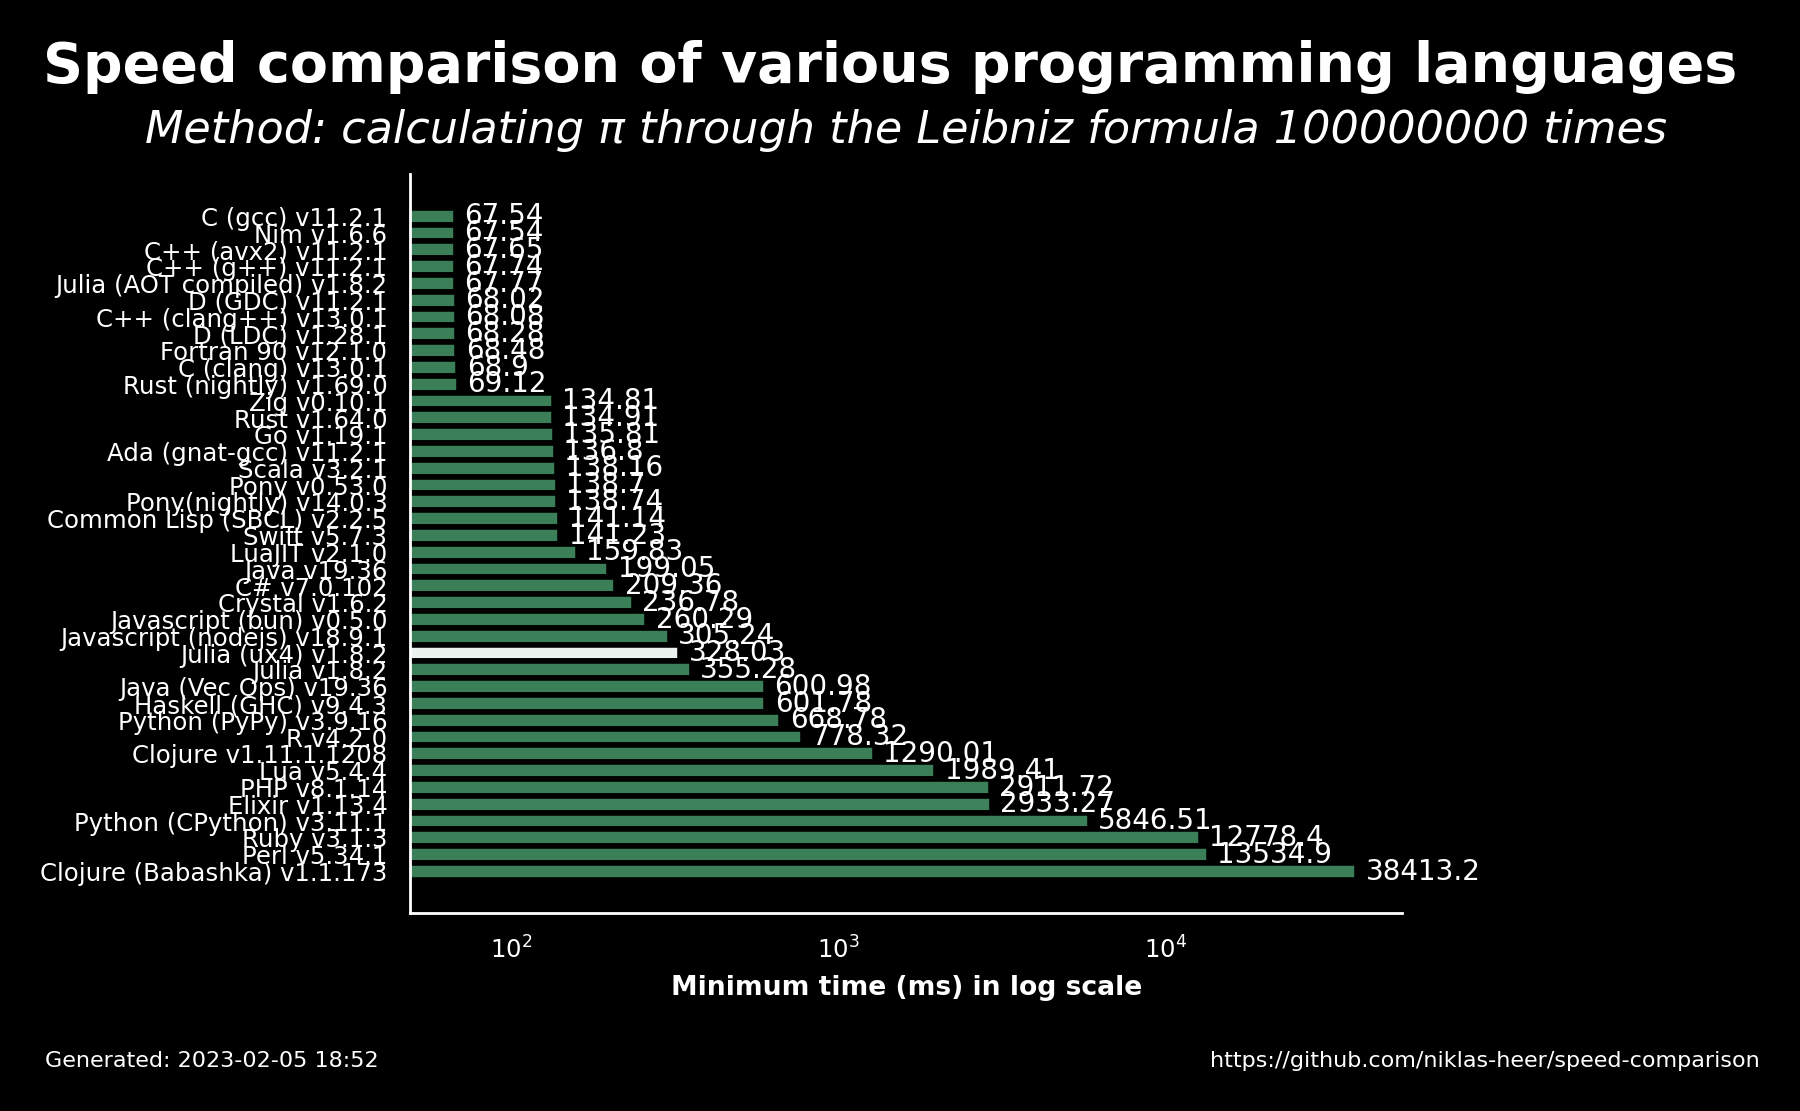
\includegraphics[width=0.5\textwidth]{./images/marco_teorico/Grafico/ComparacionLenguajes.png}
        \caption{Comparaci\'on de tiempo de ejecuci\'on entre diferentes lenguajes de Programaci\'on. Esta gr\'afica fue generada Heer \cite{ComparitionLanguajes}}
        \label{fig:tiempoEjecucion}
    \end{figure}
    \clearpage
    % Raspberry Pi 4
    \subsection{RasberyPi} % (fold)
\label{sub:Rasbery}
    % Parrafo 1
    En nuestro Trabajo Terminal, la Raspberry Pi 4 es la encargada de gestionar el robot y la ruta que nos da el 
        Physarum por medio de bluetooth. Por ello en esta sub secci\'on, daremos una breve introducci\'on a la Raspberry Pi 4,
        especificaciones t\'ecnicas, comparativas, etc.
    \vskip 0.5cm
    \subsubsection{Historia y evoluci\'on}
    \label{subsubsection:historiaEvolucion}
    % Parrafo 1
    La Raspberry Pi naci\'o en 2006 como un proyecto ideado por Eben Upton, Rob Mullins, Jack Lang y Alan Mycroft, 
        quienes trabajaban en la Universidad de Cambridge. La idea principal era crear una computadora de bajo costo 
        que permitiera a los estudiantes de la universidad mejorar sus habilidades de programaci\'on. \cite{Santamaria2023}
        En 2009, el proyecto se convirti\'o en una fundaci\'on sin fines de lucro, la Raspberry Pi Foundation, 
        con el objetivo de promover la ense\~nanza de la inform\'atica en las escuelas y pa\'ises en desarrollo. \cite{Santamaria2023}
    \vskip 0.5cm
    % Parrafo 2
    La primera Raspberry Pi fue lanzada en febrero de 2012, con un procesador ARM11 de 700 MHz, 512 MB de RAM y 
        un precio de 35 d\'olares. Desde entonces, la Raspberry Pi ha evolucionado hasta convertirse en una 
        plataforma de desarrollo muy popular, con millones de unidades vendidas en todo el mundo.\cite{Santamaria2023}
        La Raspberry Pi 4, lanzada en junio de 2019, es la versi\'on m\'as reciente de la placa y cuenta con un 
        procesador ARM Cortex-A72 de 1.5 GHz, hasta 8 GB de RAM y soporte para pantallas 4K. \cite{Santamaria2023}
    \vskip 0.5cm
    % Parrafo 3
    La Raspberry Pi ha sido utilizada en una amplia variedad de proyectos, desde servidores web y centros multimedia 
        hasta robots y sistemas de control. Su bajo costo y su flexibilidad la han convertido en una herramienta 
        muy popular entre los aficionados a la inform\'atica y la electr\'onica. Adem\'as, la Raspberry Pi ha sido 
        utilizada en proyectos educativos en todo el mundo, ayudando a ense\~nar a los j\'ovenes las habilidades 
        necesarias para el siglo XXI.
    \begin{itemize}
        \item \textbf{Raspberry Pi Model B}: La Raspberry Pi Model B es la primera versi\'on de la placa, 
            lanzada en febrero de 2012. Cuenta con un procesador ARM11 de 700 MHz, 512 MB de RAM, 
            1 puerto USB tipo A, 1 conector GPIO de 8 pines, salida HDMI, salida de audio y un lector de tarjetas SD \cite{Santamaria2023}
        \item \textbf{Raspberry Pi Model A+}: La Raspberry Pi Model A+ es una versi\'on m\'as peque\~na y 
            econ\'omica de la placa, lanzada en noviembre de 2014. Cuenta con un procesador ARM11 de 700 MHz, 
            512 MB de RAM, 1 puerto USB tipo A, 1 conector GPIO de 40 pines, salida HDMI y salida de audio 3.5 mm \cite{Santamaria2023}
        \item \textbf{Raspberry Pi 2 Model B}: La Raspberry Pi 2 Model B es la segunda versi\'on de la placa, 
            lanzada en febrero de 2015. Cuenta con un procesador ARM Cortex-A7 de 900 MHz, 1 GB de RAM, 
            4 puertos USB tipo A 2.0, 1 conector GPIO de 40 pines, salida HDMI, salida de audio 3.5mm y ethernet 10/100 \cite{Santamaria2023}
        \item \textbf{Raspberry Pi Zero}: La Raspberry Pi Zero es una versi\'on m\'as peque\~na y econ\'omica 
            de la placa, lanzada en noviembre de 2015. Cuenta con un procesador ARM11 de 1 GHz, 512 MB de RAM, 
            1 puerto mini HDMI, 1 puerto micro USB OTG, 1 conector GPIO de 40 pines y HAT compatible de 40 pines \cite{Santamaria2023} 
        \item \textbf{Raspberry Pi 3 Model B}: La Raspberry Pi 3 Model B es la tercera versi\'on de la placa, 
            lanzada en febrero de 2016. Cuenta con un procesador ARM Cortex-A53 de 1.2 GHz, 1 GB de RAM, 
            4 puertos USB tipo A 2.0, 1 conector GPIO de 40 pines, salida HDMI, salida de audio 3.5mm, ethernet 10/100, 
            conexi\'on Wifi y Bluethooth 4.1 LE \cite{Santamaria2023}
        \item \textbf{Raspberry Pi Zero W}: La Raspberry Pi Zero W es una versi\'on m\'as peque\~na y econ\'omica 
            de la placa, lanzada en febrero de 2017. Cuenta con un procesador ARM11 de 1 GHz, 512 MB de RAM, 
            1 puerto mini HDMI, 1 puerto micro USB OTG, 1 conector GPIO de 40 pines, HAT compatible de 40 pines, 
            conexi\'on Wifi y Bluethooth 4.1 LE \cite{Santamaria2023}
        \item \textbf{Raspberry Pi Zero WH}: La Raspberry Pi Zero WH es una versi\'on m\'as peque\~na y econ\'omica 
            de la placa, lanzada en febrero de 2018. Cuenta con un procesador ARM11 de 1 GHz, 512 MB de RAM, 
            1 puerto mini HDMI, 1 puerto micro USB OTG, 1 conector GPIO de 40 pines, HAT compatible de 40 pines, 
            conexi\'on Wifi y Bluethooth 4.1 LE \cite{Santamaria2023}
        \item \textbf{Raspberry Pi 3 Model B+}: La Raspberry Pi 3 Model B+ es la cuarta versi\'on de la placa,
            lanzada en marzo de 2018. Cuenta con un procesador ARM Cortex-A53 de 1.4 GHz, 1 GB de RAM, 
            4 puertos USB tipo A 2.0, 1 conector GPIO de 40 pines, salida HDMI, salida de audio 3.5mm, ethernet 10/100, 
            conexi\'on Wifi y Bluethooth 4.2 LE \cite{Santamaria2023}
        \item \textbf{Raspberry Pi 3 Model A+}: La Raspberry Pi 3 Model A+ es una versi\'on m\'as peque\~na y 
            econ\'omica de la placa, lanzada en noviembre de 2018. Cuenta con un procesador ARM Cortex-A53 de 1.4 GHz, 
            512 MB de RAM, 1 puerto USB tipo A 2.0, 1 conector GPIO de 40 pines, salida HDMI, salida de audio 3.5mm, 
            conexi\'on Wifi y Bluethooth 4.2 LE \cite{Santamaria2023}
        \item \textbf{Raspberry Pi 4 Model B}: La Raspberry Pi 4 Model B es la quinta versi\'on de la placa,
            lanzada en junio de 2019. Cuenta con un procesador ARM Cortex-A72 de 1.5 GHz, hasta 8 GB de RAM, 
            2 puertos USB tipo A 3.0, 2 puertos USB tipo A 2.0, 1 conector GPIO de 40 pines, 2 salidas micro HDMI, 
            salida de audio 3.5mm, ethernet Gigabit, conexi\'on Wifi y Bluethooth 5.0 LE \cite{Santamaria2023}
        \item \textbf{Raspberry Pi Compute Module 1}: La Raspberry Pi Compute Module 1 es una versi\'on de la placa 
            dise\~nada para su uso en sistemas embebidos, lanzada en abril de 2014. Cuenta con un procesador ARM11 de 700 MHz, 
            512 MB de RAM, 4GB eMMC Flash, Conector SODIMM DDR2 \cite{Santamaria2023}
        \item \textbf{Raspberry Pi Compute Module 3}: La Raspberry Pi Compute Module 3 es una versi\'on de la placa, 
            lanzada en enero de 2017. Cuenta con un procesador BCM2837 de cuatro n\'ucleos a 1.2 GHz, 1 GB de RAM, 4GB eMMC Flash,
            Conector SODIMM DDR2 y Conector GPIO 46 pines \cite{Santamaria2023}
        \item \textbf{Raspberry Pi Compute Module 3 Lite}: La Raspberry Pi Compute Module 3 Lite es una versi\'on de la placa,
            lanzada en enero de 2017. Cuenta con un procesador BCM2837 de cuatro n\'ucleos a 1.2 GHz, 1 GB de RAM,
            Conector SODIMM DDR2 y Conector GPIO 46 pines \cite{Santamaria2023}
        \item \textbf{Raspberry Pi Compute Module 3+}: La Raspberry Pi Compute Module 3+ es una versi\'on de la placa,
            lanzada en enero de 2019. Cuenta con un procesador BCM2837B0 de cuatro n\'ucleos a 1.2 GHz, 1 GB de RAM, 8GB, 16GB y 32 GB eMMC Flash,
            slot MicroSDHC y Conector GPIO 46 pines \cite{Santamaria2023}
        \item \textbf{Raspberry Pi Compute Module 4}: La Raspberry Pi Compute Module 4 es una versi\'on de la placa,
            lanzada en octubre de 2020. Cuenta con un procesador ARM a 1.5 GHz, 1 GB, 2 GB, 4 GB, 8 GB de RAM,
            2 puertos Gigabit Ethernet, Conectividad Wi-Fi (opcional), 1 USB C y conector GPIO de 28 pines \cite{Santamaria2023}
        \item \textbf{Raspberry Pi 400}: La Raspberry Pi 400 es una versi\'on de la placa, lanzada en noviembre de 2020.
            Cuenta con un procesador ARM Cortex-A72 de 1.5 GHz y soporte de 64 bits, 1-8 GB de RAM, 2 puertos USB tipo A 3.0, 2 puertos USB tipo A 2.0,
            Conector GPIO de 40 pines, 2 salidas micro HDMI, salida de audio 3.5mm, ethernet Gigabit, conexi\'on Wifi y Bluethooth 5.0 LE \cite{Santamaria2023}
        \item \textbf{Raspberry Pi Pico}: La Raspberry Pi Pico es una placa de desarrollo, lanzada en enero de 2021.
            Cuenta con un procesador RP2040 de doble n\'ucleo ARM Cortex-M0+ a 133 MHz, 264 KB de RAM, 2 MB de memoria flash QSPI,
            26 pines GPIO, 3 pines anal\'ogicos, 2 UART, 2 SPI, 2 I2C, 16 canales PWM, 1 temporizador de 12 bits y 1 temporizador de 16 bits \cite{Santamaria2023}
        \item \textbf{Raspberry Pi Zero 2 W}: La Raspberry Pi Zero 2 W es una versi\'on de la placa, lanzada en octubre de 2021.
            Cuenta con un procesador BCM2710A1 de cuatro n\'ucleos a 1.0 GHz, 512 MB de RAM, 1 puerto mini HDMI, 1 puerto micro USB OTG, 1 conector GPIO de 40 pines, HAT compatible de 40 pines,
            conexi\'on Wifi y Bluethooth 4.2 LE \cite{Santamaria2023}
        \item \textbf{Raspberry Pi 5}: La Raspberry Pi 5 es una versi\'on de la placa, lanzada en octubre de 2023. 
            Cuenta con un procesador ARM Cortex-A73 de 2.4 GHz, hasta 8 GB de RAM, Doble salida micro HDMI 4K60p, gpu VideoCore VII con soporte 
            de OpenGL ES 2.1 y Vulkan 1.2, decodificador HEVC 4K60, Bluethooth 5.0, WiFi 802.11ac, Ranura microSD de alta velocidad con soporte de SDR104, 
            2 puertos USB 3.0, 2 puertos USB 2.0, 1 puerto Gigabit Ethernet, interfaz PCIe 2.0, conexiones GPIO de 40 pines y bot\'on de encendido y apagado \cite{Santamaria2023}
    \end{itemize}
    
    \subsubsection{Comparativa}
\label{ssub:comparativa}
% Parrafo 1
    Una vez visto los modelos de Raspberry Pi, es necesario hacer una comparativa entre ellos para poder
        elegir el modelo que mejor se adapte a nuestras necesidades. En el Cuadro \ref{tab:comparacion01} se muestra
        una comparativa entre los modelos de Raspberry Pi.
    
    {\small % Esto hace que el texto de la tabla sea m\'as peque\~no
        \begin{longtable}{|p{1.8cm}|p{2.8cm}|p{1.2cm}|p{1.5cm}|p{1.5cm}|p{2.0cm}|p{2.0cm}|p{2.0cm}|}
        \caption{Comparaci\'on de los modelos de Raspberry Pi} \label{tab:comparacion01} \\
        \hline
        \textbf{Modelo} & \textbf{CPU} & \textbf{RAM} & \textbf{Puertos USB} & \textbf{GPIO} & \textbf{Salida Video} & \textbf{Red} & \textbf{Memoria} \\ \hline
        \endfirsthead

        \multicolumn{8}{c}{{\bfseries \tablename\ \thetable{} -- continuaci\'on de la p\'agina anterior}} \\
        \hline
        \textbf{Modelo} & \textbf{CPU} & \textbf{RAM} & \textbf{Puertos USB} & \textbf{GPIO} & \textbf{Salida Video} & \textbf{Red} & \textbf{Memoria} \\ \hline
        \endhead

        \hline \multicolumn{8}{|r|}{{Contin\'ua en la siguiente p\'agina}} \\ \hline
        \endfoot

        \hline
        \endlastfoot
            Model B                          & ARM11 700 MHz                 & 512 MB          & 1 tipo A                   & 8 pines           & HDMI                     & No                             & Lector SD                       \\ \hline
            Model A+                         & ARM11 700 MHz                 & 512 MB          & 1 tipo A                   & 40 pines          & HDMI, Audio 3.5mm        & No                             & No                              \\ \hline
            2 Model B                        & ARM Cortex-A7 900 MHz         & 1 GB            & 4 tipo A 2.0               & 40 pines          & HDMI, Audio 3.5mm        & Ethernet 10/100                & No                              \\ \hline
            Zero                             & ARM11 1 GHz                   & 512 MB          & mini HDMI, micro USB OTG   & 40 pines          & mini HDMI                & No                             & No                              \\ \hline
            3 Model B                        & ARM Cortex-A53 1.2 GHz        & 1 GB            & 4 tipo A 2.0               & 40 pines          & HDMI, Audio 3.5mm        & Ethernet 10/100, Wifi, BT 4.1  & No                              \\ \hline
            Zero W                           & ARM11 1 GHz                   & 512 MB          & mini HDMI, micro USB OTG   & 40 pines          & mini HDMI                & Wifi, BT 4.1                  & No                              \\ \hline
            Zero WH                          & ARM11 1 GHz                   & 512 MB          & mini HDMI, micro USB OTG   & 40 pines          & mini HDMI                & Wifi, BT 4.1                  & No                              \\ \hline
            3 Model B+                       & ARM Cortex-A53 1.4 GHz        & 1 GB            & 4 tipo A 2.0               & 40 pines          & HDMI, Audio 3.5mm        & Ethernet 10/100, Wifi, BT 4.2  & No                              \\ \hline
            3 Model A+                       & ARM Cortex-A53 1.4 GHz        & 512 MB          & 1 tipo A 2.0               & 40 pines          & HDMI, Audio 3.5mm        & Wifi, BT 4.2                  & No                              \\ \hline
            4 Model B                        & ARM Cortex-A72 1.5 GHz        & hasta 8 GB      & 2 tipo A 3.0, 2 tipo A 2.0 & 40 pines          & 2 micro HDMI             & Ethernet Gigabit, Wifi, BT 5.0 & MicroSD                         \\ \hline
            Compute Module 1                 & ARM11 700 MHz                 & 512 MB          & No                         & SODIMM DDR2       & No                       & No                             & 4GB eMMC                        \\ \hline
            Compute Module 3                 & BCM2837 1.2 GHz               & 1 GB            & No                         & GPIO 46 pines     & No                       & No                             & 4GB eMMC                        \\ \hline
            Compute Module 3 Lite            & BCM2837 1.2 GHz               & 1 GB            & No                         & GPIO 46 pines     & No                       & No                             & No                              \\ \hline
            Compute Module 3+                & BCM2837B0 1.2 GHz             & 1 GB            & No                         & GPIO 46 pines     & No                       & No                             & 8/16/32 GB eMMC                 \\ \hline
            Compute Module 4                 & ARM 1.5 GHz                   & 1/2/4/8 GB      & USB C                      & GPIO 28 pines     & No                       & 2x Ethernet Gigabit, Wifi (opc) & No                              \\ \hline
            Pi 400                           & ARM Cortex-A72 1.5 GHz        & 1-8 GB          & 2 tipo A 3.0, 2 tipo A 2.0 & 40 pines          & 2 micro HDMI             & Ethernet Gigabit, Wifi, BT 5.0 & No                              \\ \hline
            Pico                             & RP2040 ARM Cortex-M0+ 133 MHz & 264 KB          & No                         & 26 GPIO           & No                       & No                             & 2 MB flash                      \\ \hline
            Zero 2 W                         & BCM2710A1 1.0 GHz             & 512 MB          & mini HDMI, micro USB OTG   & 40 pines          & mini HDMI                & Wifi, BT 4.2                  & No                              \\ \hline
            Pi 5                             & ARM Cortex-A73 2.4 GHz        & hasta 8 GB      & 2 USB 3.0, 2 USB 2.0       & 40 pines          & Doble micro HDMI 4K60p   & Ethernet Gigabit, Wifi, BT 5.0 & MicroSD SDR104                  \\ \hline
        \end{longtable}
}
    \subsubsection{RasberyPi 4 Model B} % (fold)
\label{subsubsection:rasp4}
    % Parrafo 1
    Como ya vimos con anterioridad en la anterior subsubseccion, la Raspberry Pi 4 Model B es una computadora de placa \'unica 
        (SBC) desarrollada por la Fundaci\'on Raspberry Pi. Es la cuarta generaci\'on de la serie Raspberry Pi y fue lanzada en 
        junio de 2019. Nosotros enfatizaremos sus usos que tienen para el desarrollo de un robot aut\'onomo, como el que estamos
        desarrollando en nuestro Trabajo Terminal.
    \vskip 0.5cm
    % Parrafo 2
    Ventajas de la Raspberry Pi 4 Model B:
    \begin{itemize}
        \item \textbf{Alto Rendimiento:} El procesador Broadcom BCM2711 de cuatro n\'ucleos a 1.5GHz ofrede un rendimiento 
            significativamente mayor que las versiones anteriores de la Raspberry Pi, lo que permite ejecutar algoritmos 
            de control y navegaci\'on m\'as complejos.
        \item \textbf{Conectividad Avanzada:} La Raspberry Pi 4 Model B cuenta con dos puertos USB 3.0, dos puertos USB 2.0, 
            un puerto Gigabit Ethernet, conexi\'on Wi-Fi 802.11ac y Bluetooth 5.0, lo que facilita la comunicaci\'on con otros
            dispositivos, sensores y redes.
        \item \textbf{Flexibilidad de E/S:} La placa ofrece una amplia variedad de opciones de entrada y salida, incluyendo
            GPIO, HDMI, USB, Ethernet, Wi-Fi, Bluetooth, c\'amaras y pantallas, lo que permite conectar una gran variedad de
            sensores, actuadores y perif\'ericos.
        \item \textbf{Soporte de Software:} La Raspberry Pi 4 Model B es compatible con una amplia variedad de sistemas
            operativos, incluyendo Raspbian, Ubuntu, Windows 10 IoT Core y otros, lo que facilita el desarrollo de aplicaciones
            y la integraci\'on con otros dispositivos.
        \item \textbf{Bajo Costo:} La Raspberry Pi 4 Model B es una placa de bajo costo, lo que la hace accesible para
            estudiantes, aficionados y profesionales que deseen desarrollar proyectos de rob\'otica y automatizaci\'on.
    \end{itemize}
    \vskip 0.5cm
    % Parrafo 3
    Usos de la Raspberry Pi 4 Model B en rob\'otica:
    \begin{itemize}
        \item \textbf{Control de Robots:} La Raspberry Pi 4 Model B se puede utilizar para controlar robots m\'oviles, 
            drones, brazos rob\'oticos y otros dispositivos aut\'onomos, gracias a su alto rendimiento, conectividad avanzada
            y flexibilidad de E/S.
        \item \textbf{Visi\'on por Computadora:} La Raspberry Pi 4 Model B se puede utilizar para procesar im\'agenes y 
            v\'ideos en tiempo real, lo que permite a los robots detectar objetos, seguir l\'ineas, evitar obst\'aculos y 
            realizar otras tareas de visi\'on por computadora.
        \item \textbf{Aprendizaje Autom\'atico:} La Raspberry Pi 4 Model B se puede utilizar para ejecutar algoritmos de 
            aprendizaje autom\'atico y redes neuronales, lo que permite a los robots aprender de su entorno, adaptarse a 
            nuevas situaciones y mejorar su rendimiento con el tiempo.
        \item \textbf{Interacci\'on con el Entorno:} La Raspberry Pi 4 Model B se puede utilizar para interactuar con el 
            entorno f\'isico a trav\'es de sensores y actuadores, lo que permite a los robots medir la temperatura, la 
            humedad, la luz, la distancia, la velocidad y otras variables, as\'i como controlar motores, luces, pantallas 
            y otros dispositivos.
        \item \textbf{Comunicaci\'on Inal\'ambrica:} La Raspberry Pi 4 Model B se puede utilizar para comunicarse de forma 
            inal\'ambrica con otros dispositivos, sensores y redes, lo que permite a los robots enviar y recibir datos, 
            comandos y actualizaciones de forma remota.
    \end{itemize}
    \vskip 0.5cm
    % Parrafo 4
    Por todo lo anteriormente mencionado, la Raspberry Pi 4 Model B es una excelente opci\'on para el desarrollo de un robot 
        aut\'onomo, ya que ofrece un alto rendimiento, conectividad avanzada, flexibilidad de E/S, soporte de software y bajo 
        costo, lo que la hace accesible para estudiantes, aficionados y profesionales que deseen desarrollar proyectos de rob\'otica 
        y automatizaci\'on.

    % Cubelets
    %\subsection{Cubelets}
\label{subsection:cubelets}

    % Parrafo 1
    Para el desarrollo de nuestro Trabajo Terminal, adem\'as de hacer el dise\~no para
        un robot que simule el comportamiento del Physarum Polycephalum, se decidi\'o
        utilizar los Cubelets, explicaremos que son, como funcionan, sus tipos y
        caracter\'isticas.
    \vskip 0.5cm
    \subsubsection{?`Qu\'e son los Cubelets?}
\label{ssub:queSonCubelets}
    % Parrafo 1
    Los Cubelets son un conjunto de bloques modulares que permiten a los ni\~nos y ni\~nas
        construir robots. Cada bloque tiene una funci\'on espec\'ifica, como por ejemplo
        un sensor de luz, un motor, un bloque de bater\'ia, entre otros. Los Cubelets
        se conectan f\'acilmente entre s\'i, permitiendo a los ni\~nos y ni\~nas
        construir robots de manera r\'apida y sencilla.
        
    \vskip 0.5cm
    % Parrafo 2
    Adem\'as podemos extrapolar el uso de los Cubelets a niveles de educaci\'on superior y
        profesional, ya que los Cubelets son una excelente herramienta para prototipar
        r\'apidamente robots y experimentar con diferentes configuraciones. Los Cubelets
        son una excelente herramienta para prototipar r\'apidamente robots y experimentar
        con diferentes configuraciones.
    
    \subsubsection{?`C\'omo funcionan los Cubelets?}
\label{ssub:comofuncionan}
    % Parrafo 1
    Al ser tecnolog\'ia de tipo privativa y no contar con un manual de usuario, la informaci\'on
        sobre el funcionamiento interno de los Cubelets es limitada. Sin embargo, podemos
        inferir su funcionamiento a partir de la informaci\'on proporcionada por la p\'agina
        oficial de Cubelets\cite{modrobotics2023} y de nuestra propia observaci\'on.
    \vskip 0.5cm
    % Parrafo 2
    Para empezar, lo fundamental es que son piezas cuadradas hechas de pl\'astico que 
        dentro de su estructura cuentan con un microcontrolador, que a su vez tiene 
        programado su propia libreria de funciones, por ejemplo, tenemos la librer\'ia 
        'cubelet.h' y 'led.h' que nos permiten controlar ciertos aspectos dentro de los cubelets.\cite{modrobotics2012}
    \vskip 0.5cm
    % Parrafo 3
    Tambi\'es cuentan con imanes en casi cada una de sus caras, hay algunas que tienen 
        imanes en todas sus caras, otras que tinen 4 imanes en sus caras y en la otra caracter
        tienen su 'funci\'on especial' como por ejemplo el cubelet sensor de luz, como su nombre lo 
        sugiere es un sensor de luz, pero tambi\'en cuenta con un im\'an en una de sus caras.
    \vskip 0.5cm
    % Parrafo 4
    Tambi\'en cabe a\~nadir que el desarrollo en cuanto a c\'odigo es bastante limitado por lo que 
        nos dejen hacer las librerias de los cubelets y las librerias \'estandar de C, sin embargo 
        se con estos pocas acciones que podemos programar en cada uno de los cubelets, podemos
        hacer que los cubelets interactuen entre s\'i provocando comportamientos complejos.
    \subsubsection{Tipos y Caracter\'isticas}
\label{ssub:tiposYCaractCubelets}
    % Parrafo 1
    A continuaci\'on mencionaremos los tipos de Cubelets que existen y sus caracter\'isticas, estos fueron extraidos de la p\'agina ofical de los
        cubelets \cite{modrobotics2023}.
    \begin{itemize}
        \begin{minipage}
            {0.5\textwidth}
            \item \textbf{Cubelet de Gr\'afico de barras}: Muestra el valor del bloque en el gr\'afico
                de barras luminoso de 10 segmentos. El valor se adapta de 0 a 255, y se visualiza en 10 
                segmentos de 25.5 cada uno.
        \end{minipage}
        \begin{minipage}
            {0.5\textwidth}
            \centering
            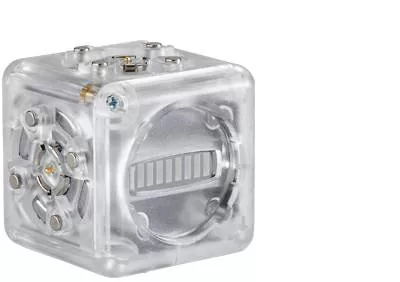
\includegraphics[width=0.5\textwidth]{./images/marco_teorico/cubelets/graficoDeBarras.png}
        \end{minipage}
        \begin{minipage}
            {0.5\textwidth}
            \item \textbf{Cubelet de Bater\'ia}: Da energ\'ia a los Cubelets conectados a \'el. 
                La bater\'ia se recarga a trav\'es de un puerto micro USB.
        \end{minipage}
        \begin{minipage}
            {0.5\textwidth}
            \centering
            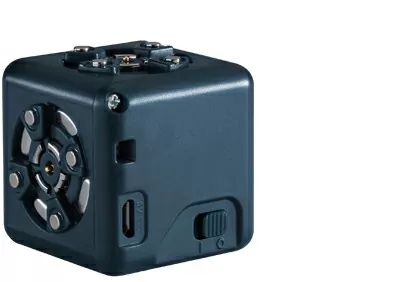
\includegraphics[width=0.5\textwidth]{./images/marco_teorico/cubelets/bateria.png}
        \end{minipage}
        \begin{minipage}
            {0.5\textwidth}
            \item \textbf{Cubelet Bloquedor}: Bloquea el flujo de datos de sus vecinos.
                Permite el paso de energ\'ia pero no de datos.
        \end{minipage}
        \begin{minipage}
            {0.5\textwidth}
            \centering
            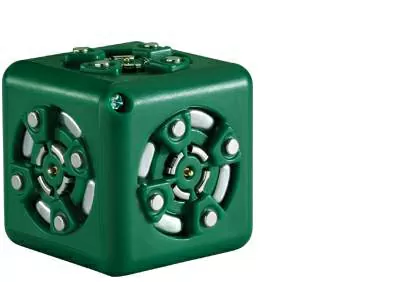
\includegraphics[width=0.5\textwidth]{./images/marco_teorico/cubelets/bloqueador.png}
        \end{minipage}
        \begin{minipage}
            {0.5\textwidth}
            \item \textbf{Cubelet de Bluethooth}: Permite la comunicaci\'on inal\'ambrica entre
                los Cubelets y otros dispositivos. Sin embargo esto solo lo hace para programar el 
                comportamiento de los Cubelets, no para la transmisi\'on de datos.
        \end{minipage}
        \begin{minipage}
            {0.5\textwidth}
            \centering
            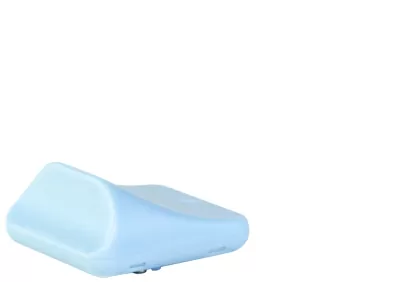
\includegraphics[width=0.5\textwidth]{./images/marco_teorico/cubelets/bluetooth.png}
        \end{minipage}
        \begin{minipage}
            {0.5\textwidth}
            \item \textbf{Cubelet de Sensor de Luz}: Mide la intensidad de la luz en su entorno.
        \end{minipage}
        \begin{minipage}
            {0.5\textwidth}
            \centering
            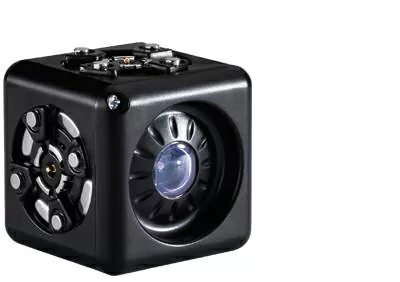
\includegraphics[width=0.5\textwidth]{./images/marco_teorico/cubelets/sensorDeLuz.png}
        \end{minipage}
        \begin{minipage}
            {0.5\textwidth}
            \item \textbf{Cubelet de Distancia}: Mide la distancia a un objeto en su entorno.
        \end{minipage}
        \begin{minipage}
            {0.5\textwidth}
            \centering
            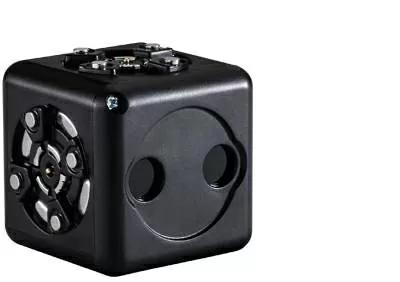
\includegraphics[width=0.5\textwidth]{./images/marco_teorico/cubelets/sensorDeDistancia.png}
        \end{minipage}
        \begin{minipage}
            {0.5\textwidth}
            \item \textbf{Cubelet de Temperatura}: Mide la temperatura en su entorno.
        \end{minipage}
        \begin{minipage}
            {0.5\textwidth}
            \centering
            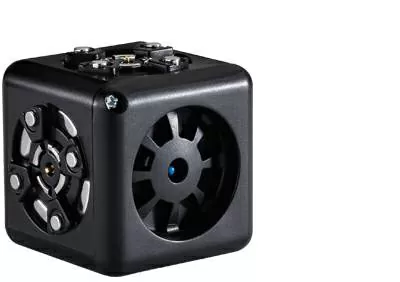
\includegraphics[width=0.5\textwidth]{./images/marco_teorico/cubelets/sensorDeTemperatura.png}
        \end{minipage}
        \begin{minipage}
            {0.5\textwidth}
            \item \textbf{Cubelet de Movimiento}: Es un cubelet que con 2 llantas y un motor, 
                permite que el robot se mueva.
        \end{minipage}
        \begin{minipage}
            {0.5\textwidth}
            \centering
            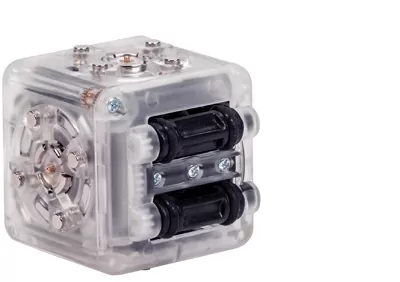
\includegraphics[width=0.5\textwidth]{./images/marco_teorico/cubelets/movimiento.png}
        \end{minipage}
        \begin{minipage}
            {0.5\textwidth}
            \item \textbf{Cubelet de Luz}: Emite luz con un led blanco y dependiendo del valor que 
                reciba, la intensidad de la luz variar\'a.
        \end{minipage}
        \begin{minipage}
            {0.5\textwidth}
            \centering
            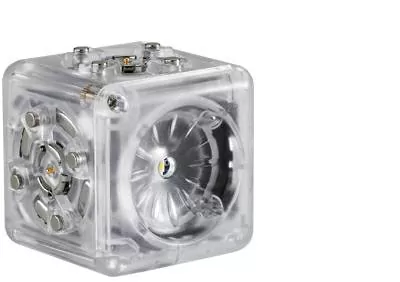
\includegraphics[width=0.5\textwidth]{./images/marco_teorico/cubelets/luz.png}
        \end{minipage}
        \begin{minipage}
            {0.5\textwidth}
            \item \textbf{Cubelet de Inversor}: Invierte el valor que recibe, es decir, si recibe un 0,
                emitir\'a un 255 y viceversa.
        \end{minipage}
        \begin{minipage}
            {0.5\textwidth}
            \centering
            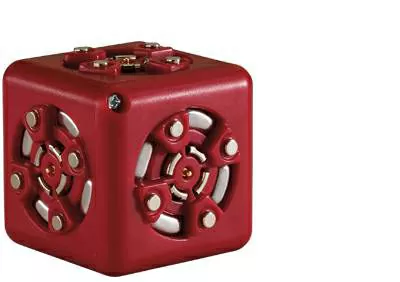
\includegraphics[width=0.5\textwidth]{./images/marco_teorico/cubelets/inversor.png}
        \end{minipage}
        \begin{minipage}
            {0.5\textwidth}
            \item \textbf{Cubelet de Perilla}: Permite ajustar el valor que recibe, es decir, si recibe
                un 0, emitir\'a un 0, si recibe un 255, emitir\'a un 255 y si recibe un valor intermedio,
                emitir\'a un valor intermedio.
        \end{minipage}
        \begin{minipage}
            {0.5\textwidth}
            \centering
            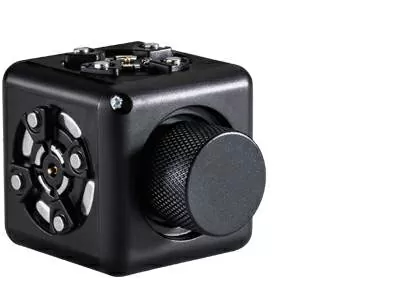
\includegraphics[width=0.5\textwidth]{./images/marco_teorico/cubelets/perilla.png}
        \end{minipage}
        \begin{minipage}
            {0.5\textwidth}
            \item \textbf{Cubelet de M\'aximo}: Emite el valor m\'as alto que recibe.
        \end{minipage}
        \begin{minipage}
            {0.5\textwidth}
            \centering
            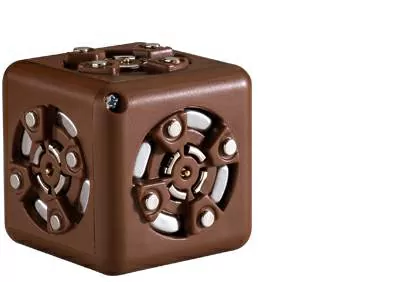
\includegraphics[width=0.5\textwidth]{./images/marco_teorico/cubelets/maximo.png}
        \end{minipage}
        \begin{minipage}
            {0.5\textwidth}
            \item \textbf{Cubelet de M\'inimo}: Emite el valor m\'as bajo que recibe.
        \end{minipage}
        \begin{minipage}
            {0.5\textwidth}
            \centering
            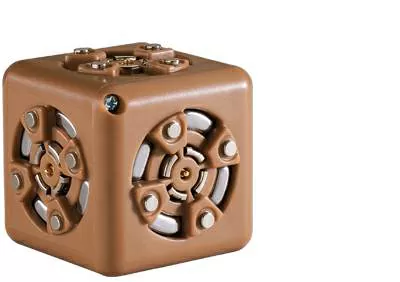
\includegraphics[width=0.5\textwidth]{./images/marco_teorico/cubelets/minimo.png}
        \end{minipage}
        \begin{minipage}
            {0.5\textwidth}
            \item \textbf{Cubelet Pasivo}: No tiene ninguna funci\'on, solo sirve para conectar los 
                Cubelets entre s\'i.
        \end{minipage}
        \begin{minipage}
            {0.5\textwidth}
            \centering
            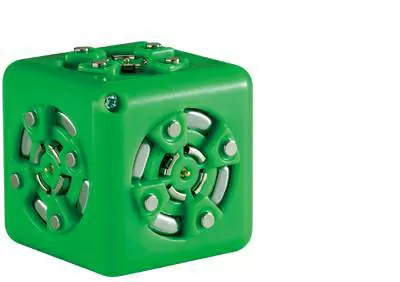
\includegraphics[width=0.5\textwidth]{./images/marco_teorico/cubelets/pasivo.png}
        \end{minipage}
        \begin{minipage}
            {0.5\textwidth}
            \item \textbf{Cubelet de Buzzer}: Emite un sonido con una frecuencia dependiendo del valor
                que recibe.
        \end{minipage}
        \begin{minipage}
            {0.5\textwidth}
            \centering
            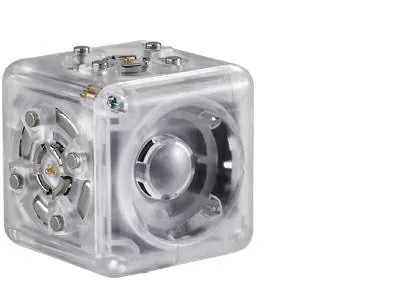
\includegraphics[width=0.5\textwidth]{./images/marco_teorico/cubelets/buzzer.png}
        \end{minipage}
        \begin{minipage}
            {0.5\textwidth}
            \item \textbf{Cubelet Rotativo}: Con un motor gira dependiendo del valor que recibe.
        \end{minipage}
        \begin{minipage}
            {0.5\textwidth}
            \centering
            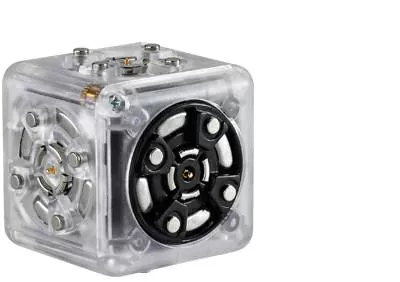
\includegraphics[width=0.5\textwidth]{./images/marco_teorico/cubelets/rotativo.png}
        \end{minipage}
        \begin{minipage}
            {0.5\textwidth}
            \item \textbf{Cubelet Umbral}:  El Threshold Cubelet es un THINK Cubelet con una perilla para alterar 
                el comportamiento de tus robots. Emitir\'a un valor de cero hasta que sus entradas superen el umbral establecido 
                por la perilla. Por encima de este umbral, los datos fluir\'an normalmente.
        \end{minipage}
        \begin{minipage}
            {0.5\textwidth}
            \centering
            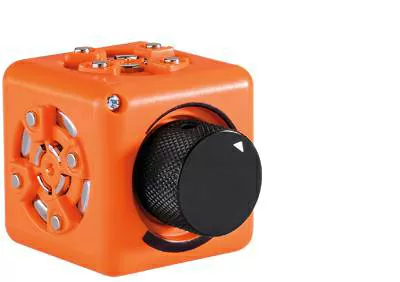
\includegraphics[width=0.5\textwidth]{./images/marco_teorico/cubelets/umbral.png}
        \end{minipage}
    \end{itemize}
    % Protocolos de comunicaci\'on
    \subsection{Protocolos de comunicaci\'on} % (fold)
\label{sub:Protocolos}
    % Parrafo 1
    La comunicaci\'on entre dispositivos es un aspecto fundamental en la rob\'otica, ya que permite la interacci\'on entre los diferentes 
        componentes de un sistema. En nuestro Trabajo Terminal, la comunicaci\'on entre el robot y el Physarum se realiza por medio de
        una aplicaci\'on m\'ovil que se comunica mediante diversos protocolos de comunicaci\'on. En esta subsecci\'on, se describir\'an
        los protocolos de comunicaci\'on utilizados en nuestro Trabajo Terminal.
    \vskip 0.5cm
    \subsubsection{WebSocket}
\label{sub:WebSocket}
    % Parrafo 1
    El protocolo de WebSocket fue desarrollado ya que el protocolo HTTP no es adecuado para aplicaciones en tiempo real, esto por que 
        el protocolo HTTP es de petici\'on-respuesta, lo que significa que el cliente debe solicitar informaci\'on al servidor y el servidor
        debe responder a la solicitud. En cambio, el protocolo WebSocket permite una comunicaci\'on bidireccional entre el cliente y el servidor,
        en otras palabras, existe una conexi\'on persistente entre el cliente y el servidor, lo que permite que el servidor env\'ie informaci\'on
        al cliente sin que este lo solicite. \cite{Kitamura2012}
    \vskip 0.5cm
        % P\'arrafo 2
        A diferencia de los protocolos de comunicaci\'on tradicionales, WebSocket permite reducir la latencia en aplicaciones que 
            requieren una actualizaci\'on constante de datos, como juegos multijugador, chats en tiempo real, o plataformas de 
            trading financiero. Esta capacidad es posible gracias al establecimiento de una conexi\'on persistente a trav\'es de 
            un \'unico canal Protocolo de Control de Transmisi\'on (Transmission Control Protocol, TCP), que permanece abierta hasta que alguna de las partes decide cerrarla. Esto reduce la sobrecarga 
            de establecer conexiones repetidas y mejora significativamente el rendimiento de las aplicaciones que requieren 
            actualizaciones constantes. \cite{RFC6455}
    \vskip 0.5cm
        % P\'arrafo 3
        El proceso de establecimiento de una conexi\'on WebSocket comienza con un "handshake" basado en HTTP, donde el cliente 
            solicita la apertura de una conexi\'on WebSocket al servidor utilizando un encabezado espec\'ifico, y el servidor 
            responde aceptando o rechazando la conexi\'on. Una vez completado el "handshake", la conexi\'on se actualiza y ambos 
            pueden intercambiar mensajes en formato binario o texto sin necesidad de seguir el ciclo de solicitud-respuesta. 
            Esto hace que WebSocket sea altamente eficiente para aplicaciones en tiempo real que manejan grandes cantidades de 
            datos o requieren baja latencia. \cite{FetteMelnikov}
    \vskip 0.5cm
        % P\'arrafo 4
        Adem\'as, WebSocket proporciona ventajas en cuanto a la reducci\'on del uso de ancho de banda. Al evitar la necesidad de 
            crear m\'ultiples conexiones y al eliminar los encabezados HTTP innecesarios en cada intercambio de mensajes, 
            se logra una transmisi\'on de datos m\'as ligera. Esto es especialmente \'util en entornos donde los recursos de red 
            son limitados, como dispositivos m\'oviles o redes con baja velocidad. \cite{WebSocketEfficiency}
    \vskip 0.5cm
        % P\'arrafo 5
        Sin embargo, aunque WebSocket ofrece muchas ventajas en t\'erminos de rendimiento y latencia, 
            su implementaci\'on puede presentar desaf\'ios de seguridad, como la exposici\'on a ataques 
            de secuestro de WebSocket entre sitios (Cross-Site WebSocket Hijacking, CSWSH) o 
            vulnerabilidades de inyecci\'on. Por esta raz\'on, es importante integrar medidas de seguridad, 
            como el uso de WebSockets sobre el protocolo de Seguridad de la Capa de Transporte 
            (Transport Layer Security, TLS), conocido como WSS para cifrar las comunicaciones, 
            y pol\'iticas adecuadas de validaci\'on del origen de las conexiones \cite{WebSocketSecurity}.
    
    \subsubsection{HTTP} % (fold)
\label{ssub:HTTP}

    El protocolo HTTP (Hypertext Transfer Protocol) es un protocolo de comunicaci\'on utilizado en 
        la World Wide Web para la transferencia de informaci\'on entre un cliente y un servidor. 
        Fue dise\~nado para ser un protocolo simple y flexible, que permitiera la transferencia 
        de datos de manera eficiente y segura. \cite{RFC2616}
    \vskip 0.5cm
        % P\'arrafo 2
        HTTP opera bajo el modelo petici\'on-respuesta, donde el cliente env\'ia una petici\'on al servidor 
            solicitando un recurso espec\'ifico, y el servidor responde con el recurso solicitado o un c\'odigo 
            de estado que indica si la petici\'on fue exitosa o no. Las peticiones y respuestas en HTTP est\'an 
            compuestas por un conjunto de encabezados y opcionalmente un cuerpo de mensaje, que contiene la 
            informaci\'on a transferir. \cite{RFC2616}
    \vskip 0.5cm
        % P\'arrafo 3
        HTTP es un protocolo sin estado, lo que significa que cada petici\'on se procesa de manera independiente, 
            sin tener en cuenta las peticiones anteriores. Esto permite que el servidor sea m\'as escalable y 
            flexible, ya que no necesita mantener un estado de sesi\'on con cada cliente. Sin embargo, esta 
            caracter\'istica tambi\'en implica que el servidor no puede recordar informaci\'on sobre el cliente 
            entre peticiones, lo que puede limitar la interacci\'on entre el cliente y el servidor. \cite{RFC2616}
    \vskip 0.5cm
        % P\'arrafo 4
        HTTP utiliza el protocolo TCP (Transmission Control Protocol) como su capa de transporte, lo que garantiza 
            una comunicaci\'on fiable y ordenada entre el cliente y el servidor. Las conexiones HTTP se establecen 
            mediante un \textit{handshake} entre el cliente y el servidor, donde se negocian los par\'ametros de la 
            conexi\'on, como el tipo de contenido aceptado, la codificaci\'on de transferencia, y la longitud del 
            cuerpo del mensaje. Una vez establecida la conexi\'on, el cliente y el servidor pueden intercambiar 
            mensajes de manera eficiente y segura. \cite{RFC2616}
    \vskip 0.5cm
        % P\'arrafo 5
        A pesar de su simplicidad y flexibilidad, HTTP tiene algunas limitaciones en t\'erminos de rendimiento y 
            eficiencia. Por ejemplo, HTTP es un protocolo de texto plano, lo que significa que los mensajes enviados 
            a trav\'es de HTTP deben ser codificados en texto legible por humanos, lo que puede aumentar el tama\~no 
            de los mensajes y reducir la eficiencia de la transferencia de datos. Adem\'as, HTTP no es adecuado para 
            aplicaciones en tiempo real, ya que su modelo petici\'on-respuesta puede introducir latencia en la 
            comunicaci\'on entre el cliente y el servidor. \cite{RFC2616}
    \vskip 0.5cm
        % P\'arrafo 6
        A pesar de estas limitaciones, HTTP sigue siendo uno de los protocolos de comunicaci\'on m\'as utilizados en 
            la World Wide Web, debido a su simplicidad, flexibilidad y compatibilidad con una amplia variedad de 
            plataformas y tecnolog\'ias. Sin embargo, en aplicaciones que requieren una comunicaci\'on m\'as eficiente 
            y en tiempo real, es posible que sea necesario utilizar protocolos m\'as especializados, como WebSocket o 
            MQTT, que est\'an dise\~nados espec\'ificamente para este prop\'osito. \cite{RFC2616}
% subsubsection HTTP (end)
    \subsubsection{Comunicaci\'on en Tiempo Real en la Web (Web Real-Time Communication, WebRTC)} % (fold)
\label{ssub:WebRTC}

    %Parrafo 1
    Comunicaci\'on en Tiempo Real en la Web (Web Real-Time Communication, WebRTC) es un conjunto de tecnolog\'ias que permite la comunicaci\'on en tiempo real entre navegadores web 
        y aplicaciones m\'oviles. Fue desarrollado por Google en 2011 con el objetivo de facilitar la creaci\'on de aplicaciones de 
        comunicaci\'on en tiempo real, como videollamadas, conferencias web y transmisi\'on de datos en tiempo real. \cite{WebRTC}
    \vskip 0.5cm
        % P\'arrafo 2
        WebRTC se basa en varios est\'andares abiertos, como el Protocolo de Transporte en Tiempo Real (Real-Time Transport Protocol, RTP), 
            el Protocolo de Control de Transporte en Tiempo Real (Real-Time Transport Control Protocol, RTCP) y 
            Protocolo de Descripci\'on de Sesi\'on (Session Description Protocol, SDP), que permiten la transmisi\'on 
            de datos en tiempo real a trav\'es de la web. Estos est\'andares est\'an dise\~nados para ser compatibles con una amplia 
            variedad de dispositivos y plataformas, lo que facilita la creaci\'on de aplicaciones de comunicaci\'on en tiempo real 
            que funcionan en diferentes entornos. \cite{WebRTC}
    \vskip 0.5cm
        % P\'arrafo 3
        Una de las caracter\'isticas m\'as importantes de WebRTC es su capacidad para establecer conexiones punto a punto entre 
            los clientes, lo que permite una comunicaci\'on directa y segura entre los usuarios sin necesidad de pasar por un 
            servidor centralizado. Esto reduce la latencia y mejora la calidad de la comunicaci\'on, ya que los datos se transmiten 
            directamente entre los clientes sin intermediarios. Adem\'as, al utilizar cifrado de extremo a extremo, WebRTC garantiza 
            la privacidad y seguridad de las comunicaciones, protegiendo los datos de posibles ataques o interceptaciones. \cite{WebRTC}
    \vskip 0.5cm
        % P\'arrafo 4
        WebRTC es compatible con una amplia variedad de dispositivos y plataformas, incluyendo navegadores web, aplicaciones m\'oviles 
            y dispositivos Internet de las Cosas (Internet of Things, IoT), lo que lo convierte en una soluci\'on vers\'atil para la creaci\'on de aplicaciones 
            de comunicaci\'on en tiempo real en diferentes entornos. Adem\'as, al ser un est\'andar abierto, WebRTC est\'a respaldado por 
            una amplia comunidad de desarrolladores y empresas, lo que garantiza su compatibilidad y soporte a largo plazo. \cite{WebRTC}

% subsubsection WebRTC (end)
% subsection Protocolos (end)
